\documentclass[10pt]{CSUN}
%%%packages%%%
\usepackage[latin1]{inputenc}
%\usepackage{newcent}
\usepackage{verbatim}
\usepackage{graphicx}
\usepackage{amsmath}
\usepackage{amsfonts}
\usepackage{amssymb}
\usepackage{amsthm}
\usepackage[section]{placeins}
\usepackage{listings}%R Code
\usepackage{color}%R code
\usepackage{tikz}
\usetikzlibrary{patterns}
% \usepackage{tkz-graph}
% \usepackage{tkz-berge}
% \usepackage{tkz-euclide}
% \usepackage{hyperref}
%\usepackage[left=1in, right=1in, top=.9in, bottom=.9in]{geometry}
\usepackage{setspace}
%\usepackage{hyperref}
\usepackage{pdflscape}
\usepackage[english]{babel}
\usepackage{times}
\usepackage[T1]{fontenc}
\usepackage{multirow}
\usepackage{mathptmx}
%\usepackage[hidelinks]{hyperref}
\usepackage{lipsum}
\usepackage{titletoc}
\usepackage[toc,page]{appendix}
\usepackage{appendix}
\usepackage{enumerate}
\usepackage{enumitem}
%\usepackage{subfigure}
\usepackage{caption}
\usepackage{subcaption}

%%CSUN Stuff%%%
\titlecontents{chapter}
  [0em]
   {\bfseries \addvspace{\baselineskip}}
  {\linebreak \rmfamily \chaptername\hspace{.1em} \thecontentslabel\quad \newline  }
  {\rmfamily}
  {\titlerule*[1pc]{.}\contentspage}

\titlecontents{section}
[1em]
   {}
  {\thecontentslabel \hspace{1em}}
   {}
    {\titlerule*[1pc]{.}\contentspage}

\titlecontents{subsection}
[3.3em]
   {}
  {\thecontentslabel \hspace{1.3em}}
   {}
    {\titlerule*[1pc]{.}\contentspage}

% for bibliography, abstract etc

\titlecontents{part}
  [0em]
   {\rmfamily \addvspace{\baselineskip}}
  {\linebreak \rmfamily \chaptername\hspace{.1em} \thecontentslabel\quad \newline  }
  {\rmfamily}
  {\titlerule*[1pc]{.}\contentspage}


\titlecontents{subsubsection}
[0em]
   {{\rmfamily \addvspace{\baselineskip}}}
  {\thecontentslabel \hspace{1em}}
   {}
    {\titlerule*[1pc]{}}
%%%END OF CSUN STUFF%%%
%%%theoerms, etc%%%%
\theoremstyle{plain}% default
\newtheorem{thm}{Theorem}[section]
\newtheorem{prop}{Proposition}[section]
\newtheorem{lem}{Lemma}[section]
\newtheorem{pf}{Proof}[section]
\theoremstyle{definition}
\newtheorem{definition}{Definition}[section]
\newtheorem{example}{Example}[section]
\theoremstyle{remark}
\newtheorem{rmk}{Remark}[section]
\newtheorem{case}{Case}
\newtheorem{prob}{Problem}[section]
%%%% R Code%%%%
\definecolor{dkgreen}{rgb}{0,0.6,0}
\definecolor{gray}{rgb}{0.5,0.5,0.5}
\definecolor{mauve}{rgb}{0.58,0,0.82}
\lstset{frame=tb,
  language=R,
  aboveskip=3mm,
  belowskip=3mm,
  showstringspaces=false,
  columns=flexible,
  basicstyle={\small\ttfamily},
  numbers=none,
  numberstyle=\tiny\color{gray},
  keywordstyle=\color{blue},
  commentstyle=\color{dkgreen},
  stringstyle=\color{mauve},
  breaklines=true,
  breakatwhitespace=true
  tabsize=3
}

%%%%%%%%TikZ Commands

\def\hexagonsize{1cm}
\pgfdeclarepatternformonly
  {hexagons}% name
  {\pgfpointorigin}% lower left
  {\pgfpoint{3*\hexagonsize}{0.866025*2*\hexagonsize}}%  upper right
  {\pgfpoint{3*\hexagonsize}{0.866025*2*\hexagonsize}}%  tile size
  {% shape description
   \pgfsetlinewidth{0.4pt}
   \pgftransformshift{\pgfpoint{0mm}{0.866025*\hexagonsize}}
   \pgfpathmoveto{\pgfpoint{0mm}{0mm}}
   \pgfpathlineto{\pgfpoint{0.5*\hexagonsize}{0mm}}
   \pgfpathlineto{\pgfpoint{\hexagonsize}{-0.866025*\hexagonsize}}
   \pgfpathlineto{\pgfpoint{2*\hexagonsize}{-0.866025*\hexagonsize}}
   \pgfpathlineto{\pgfpoint{2.5*\hexagonsize}{0mm}}
   \pgfpathlineto{\pgfpoint{3*\hexagonsize+0.2mm}{0mm}}
   \pgfpathmoveto{\pgfpoint{0.5*\hexagonsize}{0mm}}
   \pgfpathlineto{\pgfpoint{\hexagonsize}{0.866025*\hexagonsize}}
   \pgfpathlineto{\pgfpoint{2*\hexagonsize}{0.866025*\hexagonsize}}
   \pgfpathlineto{\pgfpoint{2.5*\hexagonsize}{0mm}}
   \pgfusepath{stroke}
  }
%%%%%%%%custom commands
\newcommand{\NN}{\mathbb{N}} %  set of natural numbers
\newcommand{\ZZ}{\mathbb{Z}} %  set of integer number
\newcommand{\RR}{\mathbb{R}} %  set of real numbers
\newcommand{\SH}{\mathbb{S}} %  set of unit vectors
\newcommand{\HH}{{\cal H}} %  Calligraphic H
\newcommand{\PP}{{\cal P}} %  Calligraphic P
\newcommand{\DD}{{\cal D}} %  Calligraphic D
\newcommand{\QQ}{{\cal Q}} %  Calligraphic D
\newcommand{\FF}{{\cal F}} %  Calligraphic D
\newcommand{\bbH}{{\mathbb{H}}}
\newcommand{\bbR}{{\mathbb{R}}}
\newcommand{\bbP}{{\mathbb{P}}}
\newcommand{\bbZ}{{\mathbb{Z}}}
\newcommand{\bbC}{{\mathbb{C}}}
\newcommand{\bbQ}{{\mathbb{Q}}}
\newcommand{\bbA}{{\mathbb{A}}}
\newcommand{\bbF}{{\mathbb{F}}}
\newcommand{\bbh}{{\mathbb{H}}}
\newcommand{\bbr}{{\mathbb{R}}}
\newcommand{\bbp}{{\mathbb{P}}}
\newcommand{\bbz}{{\mathbb{Z}}}
\newcommand{\bbc}{{\mathbb{C}}}
\newcommand{\bbq}{{\mathbb{Q}}}
\newcommand{\bba}{{\mathbb{A}}}
\newcommand{\bbf}{{\mathbb{F}}}
\newcommand{\bbn}{{\mathbb{N}}}
\newcommand{\bbN}{{\mathbb{N}}}
\newcommand{\disteq}{{\overset{D}{=}}}
\newcommand{\cross}{{\times}}
\newcommand{\CBeta}{{  \left( \begin{array}{c}\hat{\beta}_{1,1} - \hat{\beta}_{2,1} \\ \hat{\beta}_{1,2} -
\hat{\beta}_{2,2} \\ \vdots \\ \hat{\beta}_{1,p} - \hat{\beta}_{2,p}    \end{array} \right) }}
\newcommand{\COVW}{{\left[ \begin{array}{cc}\sigma_1^2 \left( X_1 ' X_1\right)^{-1}\\ \sigma_2^2 \left( X_2 '
X_2\right)^{-1} 
\end{array} \right]}}
\newcommand{\MSRES}{{\sigma_1^2 n_1 + \sigma_2^2 n_2 - p \left( \sigma_1^2 + \sigma_2^2 \right) }}
\newcommand{\XX}{{\left(X ' X\right)^{-1} }} 
\newcommand{\xx}{{\left(X ' X\right)^{-1} }} 
\newcommand{\ssres}{{\text{SS}_\text{RES}}}
\newcommand{\inv}[1]{{#1^{-1}}}
\renewcommand{\it}[1]{{\textit{#1}}}
% \newcommand{\iff}{{\Leftrightarrow}}
\newcommand{\comp}[2]{{\left( #1 \circ #2\right) }}
\newcommand{\set}[2]{{\left\lbrace \left.  #1 \left\vert #2  \right.\right.\right\rbrace  }}
\newcommand{\topo}{{\mathcal{T}}}
\newcommand{\powset}[1]{{\mathcal{P}\left( #1 \right) }}
%\newcommand{\vec}[1]{{\overrightarrow{#1} }}
%%%%Spacing commands %%%%%
\newcommand{\tab}{\hspace{.4cm}}
\newcommand{\quadtab}{\hspace{.4cm}}
\newcommand{\matab}{\hspace{1.01600mm}}
\renewcommand{\arraystretch}{1.5}
\newcommand{\RNum}[1]{\lowercase\expandafter{\romannumeral #1\relax}}
\newcommand{\rn}[1]{\lowercase\expandafter{(\romannumeral #1\relax)}}
\newcommand{\floor}[1]{\left\lfloor #1 \right\rfloor}
\newcommand{\ceil}[1]{\left\lceil #1 \right\rceil}
\newcommand{\combo}[2]{\left(\begin{array}{c}#1\\#2\end{array}\right)}
%\renewcommand{\baselinestretch}{1.0}
% 1.0 is for one line space, 2.0 is for double-line space, etc
%%%%Spacing commands %%%%%

%%%%Margins%%%%%% - Clinton Bowen
\setlength{\topmargin}{-.5in} 
\setlength{\textheight}{9.0in}
\setlength{\oddsidemargin}{0.5in} 
\setlength{\evensidemargin}{0.0in}
\setlength{\textwidth}{6.0in}
%%Please refer to http://en.wikibooks.org/wiki/LaTeX/Page_Layout
%%The parameters below are described pictorally on this webpage.  Tinker with the settins as needed.
%\setlength{\evensidemargin}{0cm}
%\setlength{\oddsidemargin}{0pt}
%\setlength{\topmargin}{.5in}
% \setlength{\hoffset}{0in}
% \setlength{\voffset}{0in}
% \setlength{\headheight}{0pt}
% \setlength{\headsep}{0in}%should be 1 inch from header titles
%\setlength{\textheight}{21cm}
%\setlength{\textwidth}{15.5cm}
% \setlength{\marginparsep}{0pt}
% \setlength{\marginparwidth}{0pt}
% \setlength{\footskip}{0pt}
%%%%Margins%%%%%% - Clinton Bowen
\author{Clinton Bowen}
\title{Protein Folding: Planar Configuration Spaces of Disc Arrangements and
Hinged Polygons: \textit{Protein Folding in Flatland}}
\date{April 1, 2014}
\makeindex
\begin{document}
% 
\pagenumbering{roman}
\thispagestyle{empty}
\begin{center}
CALIFORNIA STATE UNIVERSITY, NORTHRIDGE

\vspace{1.5in}
PROTEIN FOLDING: PLANAR CONFIGURATION SPACES\\
\vspace{15pt}
OF DISC ARRANGEMENTS AND HINGED POLYGONS:\\
\vspace{15pt}
PROTEIN FOLDING IN FLATLAND\\
\vspace{100pt}
A thesis submitted in partial fulfillment of the requirements\\
For the degree of Master of Science in Mathematics\\
\vspace{50pt}
By\\
\vspace{20pt}
Clinton Bowen \\
\vspace{50pt}
Spring 2014
\end{center}
\pagebreak

\addcontentsline{toc}{part}{Signature page}

\vspace*{30pt}
The thesis of Clinton Bowen is approved:

\vspace*{70pt}

\textbf{---------------------------------------------- \ \ \
\ \ \ \ \ \ \ \ \ \ \ \ \ \ ------------------}

Dr. John Dye \ \ \ \ \ \ \ \ \ \ \ \ \ \ \ \ \ \ \ \ \ \ \ \ \ \ \ \ \ \ \ \ \ \ \ \ \ \ \ \ \ \ \ \ \ \ \ \ \ \ \ \ \ \ \ \ \     Date

\vspace*{30pt}

\textbf{---------------------------------------------- \ \ \
\ \ \ \ \ \ \ \ \ \ \ \ \ \ ------------------}

Dr. Silvia Fernandez \ \ \ \ \ \ \ \ \ \ \ \ \ \ \ \ \ \ \ \ \ \ \ \ \ \ \ \ \ \ \ \ \ \ \ \ \ \ \ \ \ \ \ \ \  Date

\vspace*{30pt}

\textbf{---------------------------------------------- \ \ \
\ \ \ \ \ \ \ \ \ \ \ \ \ \ ------------------}

Dr. Bernardo Abrego \ \ \ \ \ \ \ \ \ \ \ \ \ \ \ \ \ \ \ \ \ \ \ \ \ \ \ \ \ \ \ \ \ \ \ \ \ \ \ \ \ \ \ \  Date

\vspace*{30pt}

\textbf{---------------------------------------------- \ \ \
\ \ \ \ \ \ \ \ \ \ \ \ \ \ ------------------}


Dr. Csaba Toth, Chair \ \ \ \ \ \ \ \ \ \ \ \ \ \ \ \ \ \ \ \ \ \ \ \ \ \ \ \ \ \ \ \ \ \ \ \ \ \ \ \ \ \ \ Date


\vspace*{225pt}

\begin{center}
California State University, Northridge
\end{center}

\pagebreak

\addcontentsline{toc}{part}{Dedication}
\begin{center}
DEDICATIONS
% \vspace{80pt}
% 
% To my family and friends, \\
% 
% \vspace{30pt}
% Thank you for all your support
\end{center}

\pagebreak

\addcontentsline{toc}{part}{Acknowledgement}
\begin{center}
ACKNOWLEGDEMENTS
\end{center}
\vspace{80pt}

% I would like to thank my thesis advisor Dr. Yomba and  co-chair Dr. Djellouli for their support  
% and encouragement throughout my thesis preparation.  
% Thanks also to my committee members Dr. Zakeri and Dr. Panferov. \\


\pagebreak

\renewcommand\contentsname{Table of Contents}
\tableofcontents

%\listoffigures
%\listoftables

\pagebreak
\addcontentsline{toc}{part}{Abstract}
\begin{center}
ABSTRACT \\
\vspace*{2em}
PROTEIN FOLDING: PLANAR CONFIGURATION SPACES\\
\vspace{15pt}
OF DISC ARRANGEMENTS AND HINGED POLYGONS:\\
\vspace{15pt}
PROTEIN FOLDING IN FLATLAND\\
\vspace{20pt}
By\\
\vspace{30pt}
Clinton Bowen \\
\vspace{30pt}
Master of Science in Mathematics 
\end{center}
\vspace{30pt}

Insert Abstract here


\pagebreak
\pagenumbering{arabic}
% \input{abstract}
% \begin{abstract}
We look into the decidability of whether a hinged configuration locks.
\end{abstract}
\section{Introduction}
We look into the decidability of continuity on planar configuration space using regular, unitary hexagonal polygons.  These polygons can also represent unit disk configurations \cite{Breu19983} 
\begin{figure}[ht]
\begin{center}
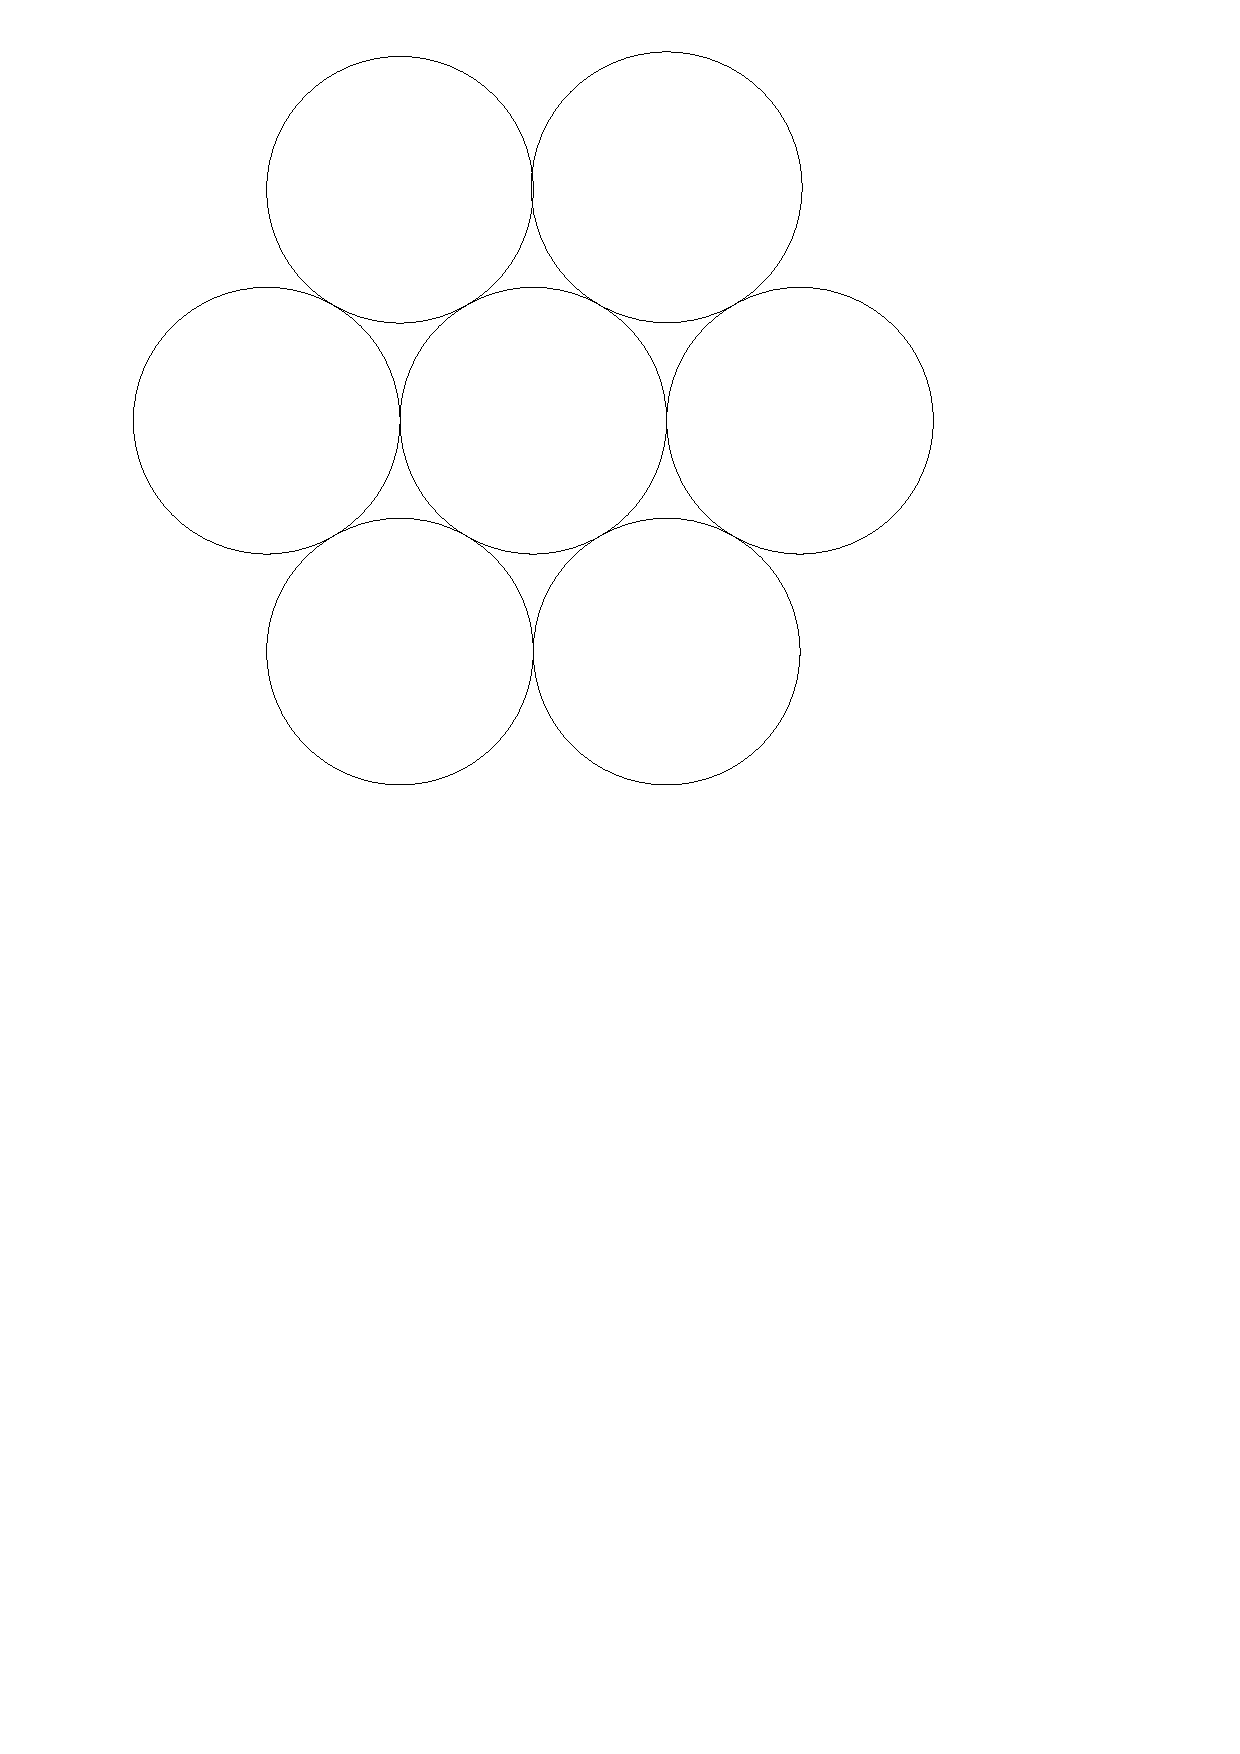
\includegraphics{graphics/7ballLocked.pdf}
\caption{A locked 7 ball configuration}
\label{figure:7ballLocked}
\end{center} 
\end{figure}
% We need the following:
% \begin{itemize}
% \item[\rn{1}] discussion on the outer configuration of hexagons
% \item[\rn{2}] discussion on the inner configuration (lattice tesselation) of hexagons the convex hull of \rn{1}
% \item[\rn{3}] discussion on the hinged cells that reside in the boundary of \rn{2}
% \item[\rn{4}] discussion on the lockedness of \rn{3} where it has two modes (boolean variable)
% \item[\rn{5}] the area of interests:
% \begin{itemize}
% \item how big are the cells of \rn{3}?
% \item does cell size matter in \rn{3}?
% \item How to form a 3-sat conjunction from a set of cells at corners of the individual hexagons within the tesselation
% \item how to form a conjunction from a set of cells on the edges of the of the hexagons.
% \end{itemize} 
% \end{itemize}  
\paragraph{Motivation}
Protein folding, graphite, crystalline structures in metallurgy.
\paragraph{Outline}
Section 2 covers the necessary mathematical concepts to understanding the
problem.  Section 3 explains the problem, Section 4 covers the results and
findings about the problem.  Section 5, the conclusion, offers final remarks on
the problem.

% \chapter{Background}

We consider four decision problems surrounding graph theory and geometry. 
The graph theory based problems involve polygonal linkages and the geometry based problems involve something called a contact graph of disks.  
In each problem, we decide whether a polygonal linkage or contact graph has a certain realization in the plane.

This thesis first presents preliminary information needed to pose our four problems, then we formally pose each problem and then provide the hardness results in all four cases.
We show that all four problems are intractable, or $\NP$ hard (see definition below). 

% \section{Problem}
\subsection{Problem Statement} text
\subsection{Decidability of Problem} test
\subsection{Locked Configuration}
Test
\begin{figure}[ht]
\begin{center}
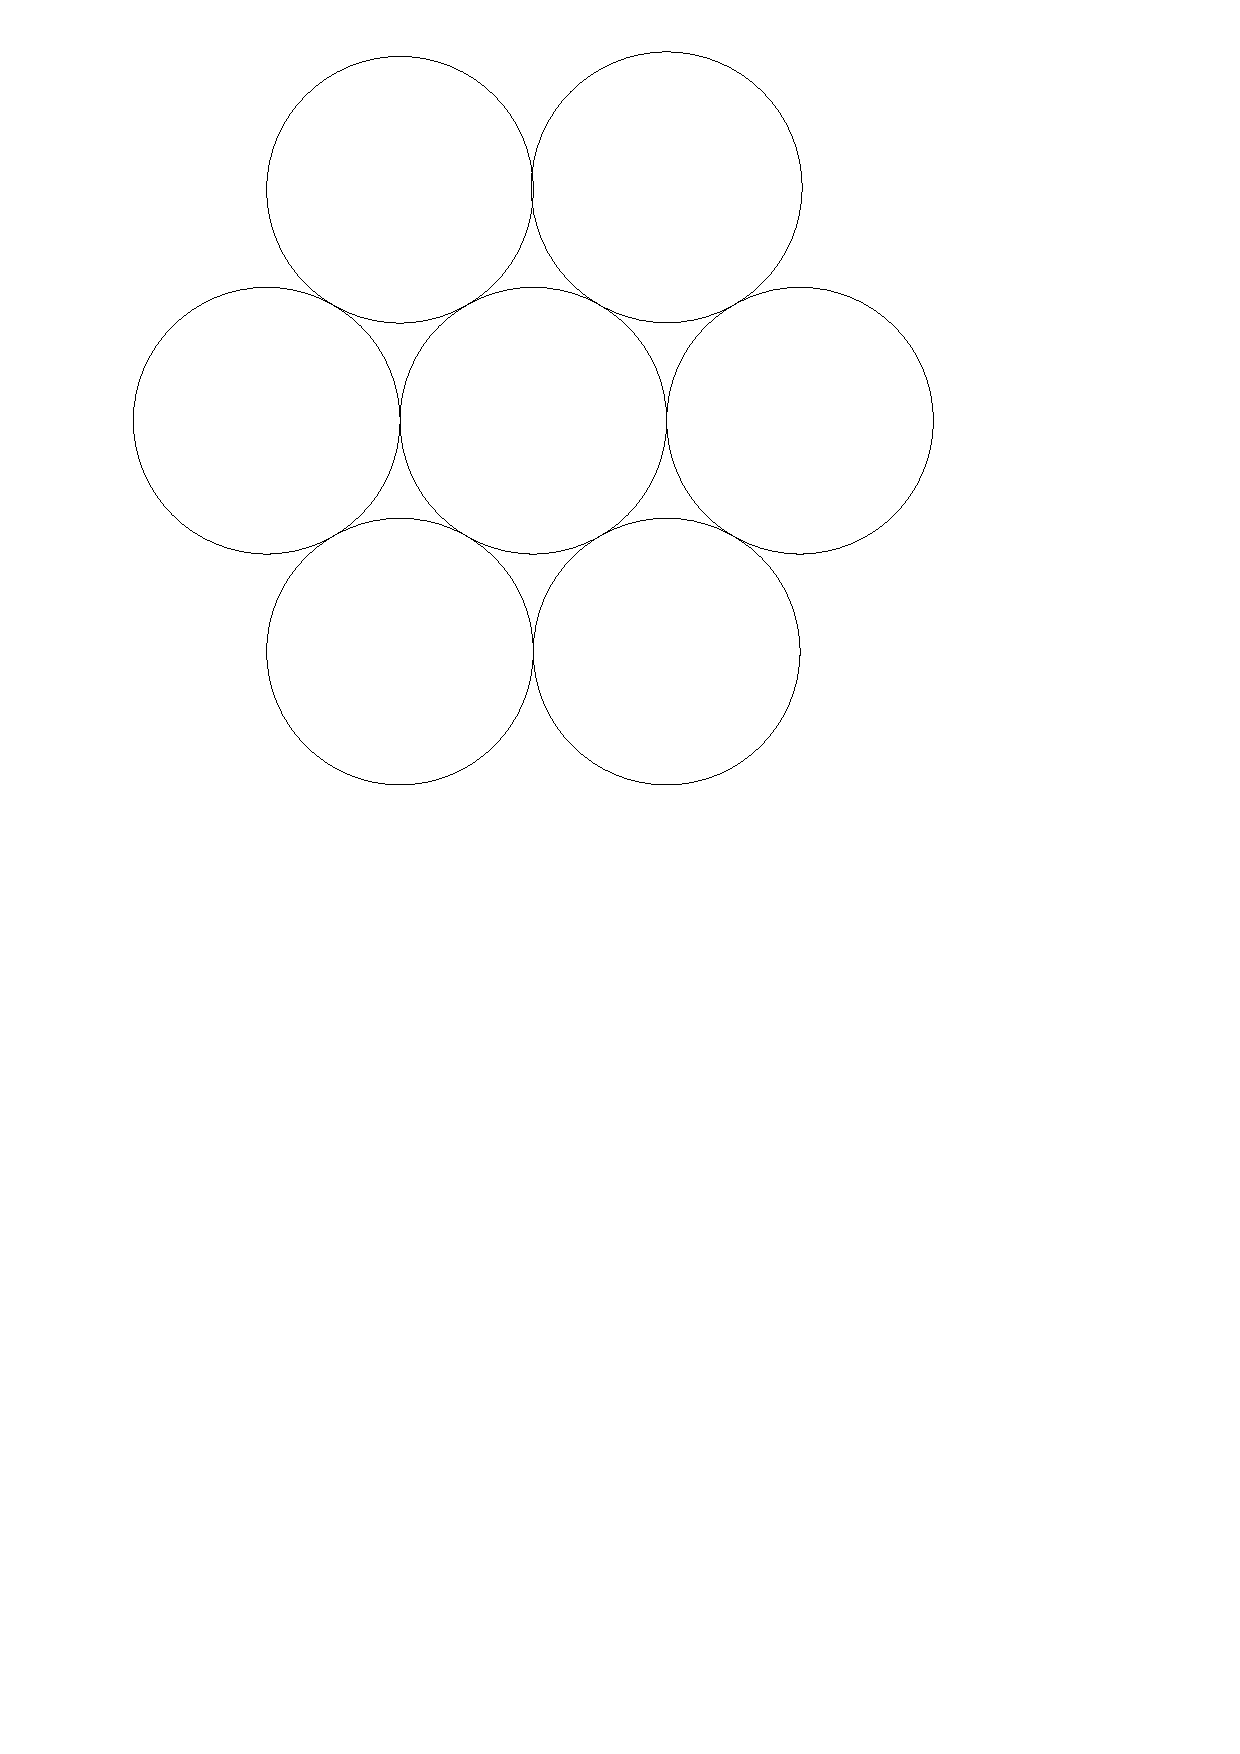
\includegraphics{graphics/7ballLocked.pdf}
\caption{A locked 7 ball configuration}
\label{figure:7ballLocked}
\end{center} 
\end{figure}
\begin{figure}[ht]
\begin{center}
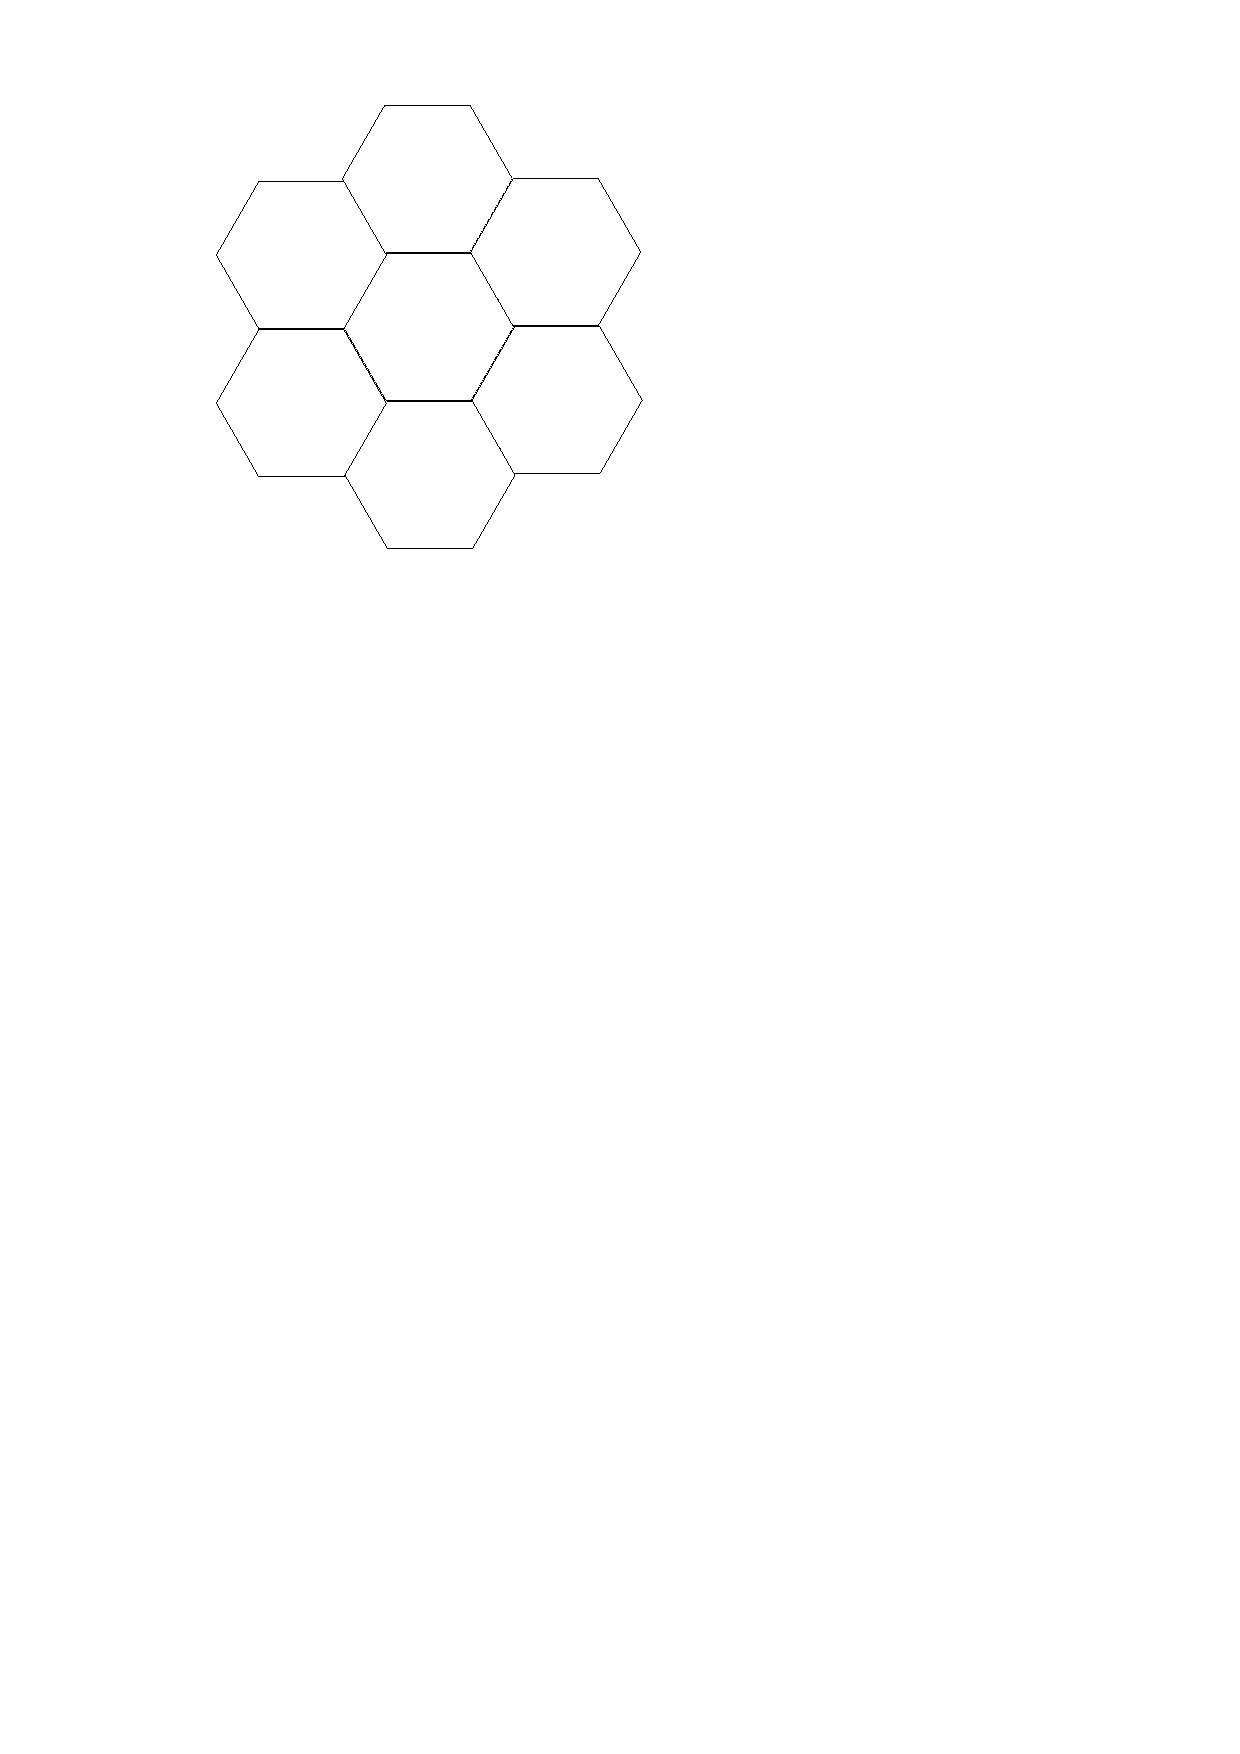
\includegraphics{graphics/7hexLocked.pdf}
\caption{A locked 7 ball configuration}
\label{figure:7hexLocked}
\end{center} 
\end{figure}
\newpage
% \input{solution}
% \section{Conclusion}
Complex structures in nature are often composed of elementary pieces that obey simple local 
composition rules. Molecular biology, nanomanufacturing, and self-assembly are prime examples. 
Mathematical models for this phenomenon typically rely on rigidity theory and formal languages. In 
this paper, we study the realizability of complex structures that are given with a local 
specification. We consider two models in Euclidean plane.

\begin{enumerate}
\item A \textbf{polygonal linkage} is a set $\PP$ of convex polygons, and a set $\HH$ of hinges,
where each hinge $h\in \HH$ corresponds to two points on the boundary of two distinct polygons.
A \emph{realization} of a polygonal linkage is an interior-disjoint placement of congruent copies 
of the polygons in $\PP$ such that the points corresponding to each hinge are identified 
(Fig.~\ref{fig:1}, left).
\item A \textbf{disk arrangement} is a set $\DD$ of pairwise interior-disjoint disks in the plane. 
The contact graph of a disk arrangement $\DD$ is a graph $G=(\DD,E)$ where two vertices are adjacent 
if the corresponding disks intersect (kiss). A \emph{realization} of a vertex-weighted graph $G$ as 
a contact graph of disks is a disk arrangement whose contact graph is $G$ and the radius of each 
disk is the corresponding vertex weight.
\end{enumerate}
\begin{figure}[htbp]
  \centering
 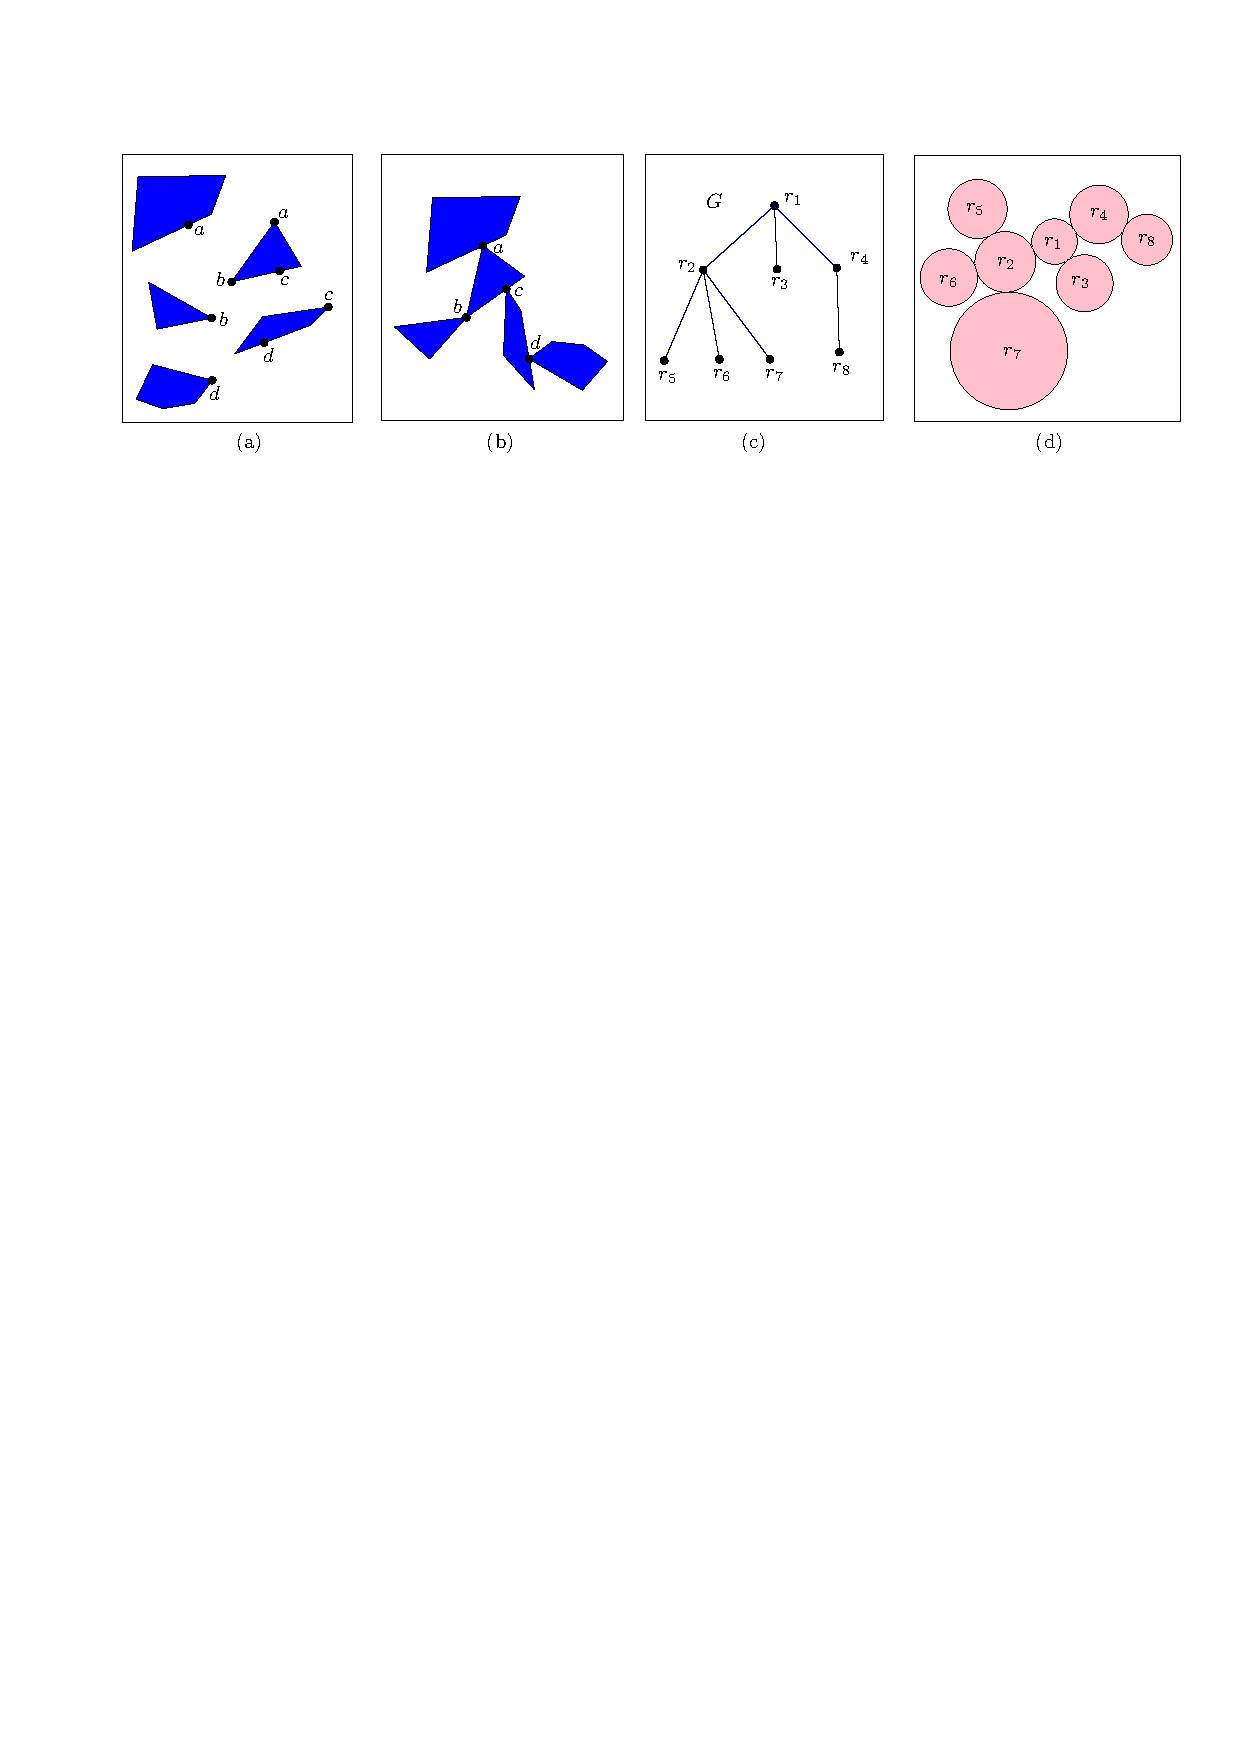
\includegraphics[width=0.95\textwidth]{graphics/fig1}
\caption{\small (a) A set of convex polygons and hinges. (b) A realization of the polygonal linkage from (a).
(c) A graph $G$ with vertex weights $r_1,\ldots, r_8$. (d) A disk arrangement that realizes the 
weighted graph $G$ as a contact graph with radii equal to the corresponding weights.}
  \label{fig:1}
\end{figure}
Each model has two variants, depending on whether \emph{reflection} is allowed for the realization 
of each piece independently. For polygonal linkages, an \emph{oriented realization} requires 
translated and rotated copies of the polygons in $\PP$ (i.e., reflection is not allowed). An 
\emph{ordered contact graph} for a disk arrangement is a \emph{plane graph} $G$, where the circular 
order of the neighbors of each vertex is specified, and an \emph{oriented realization} is disk 
arrangement with the given ordered contact graph.


\smallskip\noindent{\bf Related Previous Work.}
Polygonal linkages (or body-and-joint frameworks) are a generalization of classical linkages 
(bar-and-joint frameworks) in rigidity theory. A linkage is a graph $G=(V,E)$ with given edge 
lengths. A realization of a linkage is a (crossing-free) straight-line embedding of $G$ in the 
plane.
Bhatt and Cosmadakis~\cite{BC87} proved that the realizability of linkages is NP-hard.
Their ``logic engine'' method~\cite{SFM+11,BET+99,FHW97,HK01}, has become a powerful tool in graph 
drawing.
The logic engine is a graph composed of rigid 2-connected components, connected by cut vertices 
(hinges). The two possible realizations of each 2-connected component (that differ by a single 
reflection)  represent the truth assignment of a binary variable. This method does not applicable to 
the \emph{oriented} version of the realizability, where the circular order of the neighbors of each 
vertex is part of the input. Cabello et al.~\cite{CDR07,EW90} proved that the realizability of 
3-connected linkages (where the orientation is unique by Steinitz's theorem) is NP-hard, but 
efficiently decidable for near-triangulations~\cite{CDR07,BV96}.

Note that every \emph{tree} linkage can be realized in $\RR^2$ (with almost collinear edges). 
According to the celebrated \emph{Carpenter's Rule Theorem}~\cite{CDR03,Str05}, every realization of 
a path (or a cycle) linkage can be continuously moved (without self-intersection) to any other 
realization. In other words, the realization space of such a linkage is always connected. However, 
there are trees of maximum degree 3 with at few as 8 edges whose realization space is 
disconnected~\cite{BCD+09}; and deciding whether the realization space of a tree linkage
is connected is PSPACE-complete~\cite{AKR+04}. (Earlier, Reif~\cite{Rei79} showed that it is 
PSPACE-complete to decide whether a polygonal linkage can be moved from one realization to another 
among polygonal obstacles in $\RR^3$.) Cheong et al.~\cite{CdG+07} considers the ``inverse'' 
problems of introducing the minimum number of point obstacles to reduce the configuration space of a 
polygonal linkage to a unique realization.


Connelly et al.~\cite{CDD+10} showed that the Carpenter's Rule Theorem generalizes to certain 
polygonal linkages, which are obtained by replacing the edges of a path linkage with special 
polygons called (\emph{slender adornments}). Our Theorem~\ref{thm:hinge} indicates that if we are 
allowed to replace the edges of a path linkage with arbitrary convex polygons, then deciding whether 
the realization space is empty or not is already NP-hard.

Recognition problems for intersection graphs of various geometric object have a rich 
history~\cite{HK01}. Breu and Kirkpatrick~\cite{BK98} proved that it is NP-hard to decide whether a 
graph $G$ is the contact graph of unit disks in the plane (a.k.a. recognizing \emph{coin graphs} is 
NP-hard). A simpler proof was later provided via the logic engine~\cite{BET+99}. It is also NP-hard 
to recognize the contact graphs of pseudo-disks~\cite{HK01} and disks of bounded radii~\cite{BK95} 
in the plane, and unit disks in higher dimensions~\cite{Hli97,HK01}. All these hardness reductions 
produce graphs of high genus, and do not apply to trees. Note that the contact graphs of disks (of 
arbitrary radii) are exactly the planar graph (by Koebe's circle packing theorem), and planarity 
testing is polynomial. Consequently, every tree is the contact graph of disks of \emph{some} radii 
in the plane.

\subsection{Linkages and Polygonal Linkages}
Given a \it{graph}, an ordered pair $G = (V,E)$, comprising of a set $V$ of vertices or nodes together with a set $E$ of edges or lines, then a \it{linkage} of $G$ is the realization (or embedding) of $G$ in $\bbr^2$. A \it{polygonal linkage} is an ordered pair, $L = (H,P)$,  comprises of a set of polygons, $P$, and a set of hinge points $H$ where each hinge $h \in H$ corresponds to two points on the boundary of two distinct polygons in $P$. Without loss of generality, for this paper, we focus on linkages and polygonal linkages that are simple planar  graphs, i.e.:
\begin{itemize}
\item[\rn{1}] does not have edges (polygons) that cross (intersect),
\item[\rn{2}] have loops (i.e. $(v,v) \in E$), or
\item[\rn{3}] does not have multiple edges between any pair of vertices.
\end{itemize}
We may visit special cases in which we look at planar graphs that satisfy the last two conditions but not the first.  
\subsubsection{Configuration Spaces of Linkages}
To describe the types of motion that we are interested in linkages we must define the graph isomorphism.  Two graphs $G=(V_1,E_1)$ and $\Gamma = (V_2,E_2) $, a bijection $f: V_1 \mapsto V_2$ such that for any two vertices $u,v \in V_1$ that are adjacent, i.e. $(u, v) \in E_1$, if and only if $(f(u),f(v)) \in E_2$. 
\begin{table}[!ht]
\begin{center}
$$\begin{array}{|c|c|c|}\hline
\text{Graph}&\text{Vertices}&\text{Edges}\\\hline
G&\left\lbrace a,b,c,d,e \right\rbrace & \left\lbrace (a,b),(b,c),(c,d),(d,e),(e,a) \right\rbrace \\\hline
\Gamma&\left\lbrace 1,2,3,4,5 \right\rbrace & \left\lbrace (1,2),(2,3),(3,4),(4,5),(5,1) \right\rbrace \\\hline
\end{array} $$
\caption{Two graphs that are isomorphic with the alphabetical isomorphism $f(a)=1$, $f(b)=2$, $f(c) = 3$, $f(d)=4$, $f(e)=5$.}
\end{center} 
\label{table:linkage-1}
\end{table} 

Next we add restrictions to our graph isomorphisms to narrow our focus:
\begin{itemize}
\item[\rn{1}] We focus on isomorphisms for planar graphs and or polygonal linkages, simple planar graphs, and
\item[\rn{2}] the isomorphism preserves edge lengths (polygonal area), e.g. $d(u,v) = d(f(u),f(v))$.
\end{itemize}  
With these restrictions of our isomorphisms, we can begin to describe a range of motion to transform a linkage.  That range of motion is said to be the configuration space of that linkage.  To expand on this concept, for given linkage, $L=(V,E)$, and for a given vertex $v \in V$, the set of points in which $v$ can be realized in the plane would be the configuration space for that vertex, $C_v$.  Defining some order of the vertices in $L$, i.e. $V = \left\lbrace v_n \right\rbrace_{i=1}^n$, then the \it{configuration space} for $L$ is said to be the cartesion product of the configuration space of vertices:
\begin{equation}\label{eqn:linkages-1}
C(L) = C_{v_1} \cross C_{v_2} \cross \cdots \cross C_{v_n}
\end{equation} 
Some food for thought on configuration spaces and motions on linkages:
\begin{itemize}
\item[\rn{1}] A configuration space is said to be \it{connected} if there is a continuous mapping for any two planar realizations (linkages) of a graph in the plane.  Otherwise it is said to be \it{disconnected}.
\item[\rn{2}] If the configuration space of a vertex, $C_v$, is a singleton set, then the vertex is said to be \it{pinned}. Otherwise it is said to be \it{free}.
\item[\rn{3}] The types of motions (mappings) that we refrain from using on linkages are translations.
\end{itemize}\newpage 
%  
\section{Configuration Spaces}
\subsubsection{Confining Linkages to a Restricted Space Within a Configuration Space}
So we've covered the idea of linkages within a plane; now let's constrain the plane to a strip and have a linkage that is a \textit{polygon}, i.e. a linkage that forms a closed chain (e.g. Table \ref{table:linkage-1}), hugging the boundaries of the strip:
\begin{figure}[h]
\begin{center}
  ~ %add desired spacing between images, e. g. ~, \quad, \qquad etc.
    %(or a blank line to force the subfigure onto a new line)
  \begin{subfigure}[b]{0.49\textwidth}
	  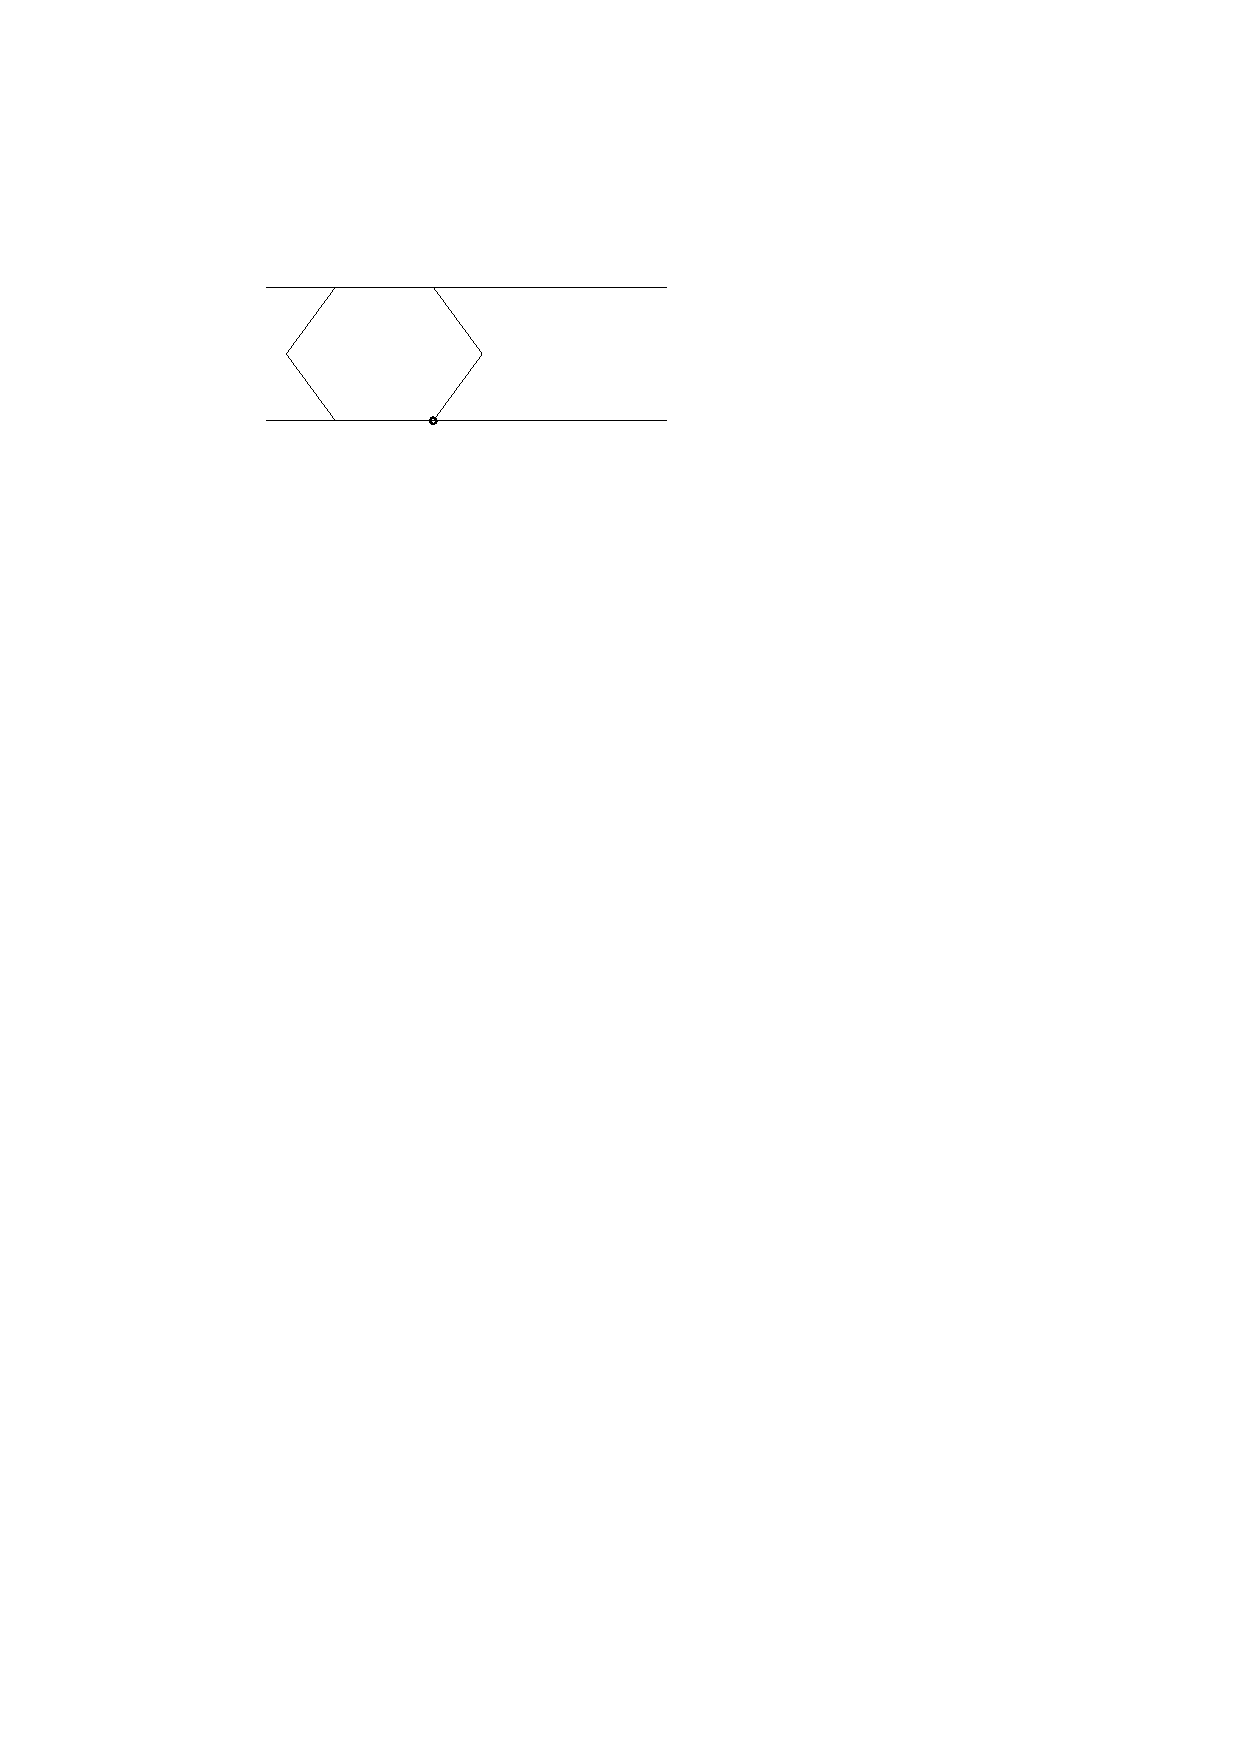
\includegraphics[width=\textwidth]{graphics/hexagonInChannelWithPinnedJointRight.pdf}
	  \caption{A bounded hexagon that resides in a channel with a pinned vertex}
	  \label{fig:linkage-1-1}
  \end{subfigure}
  \begin{subfigure}[b]{0.49\textwidth}
	  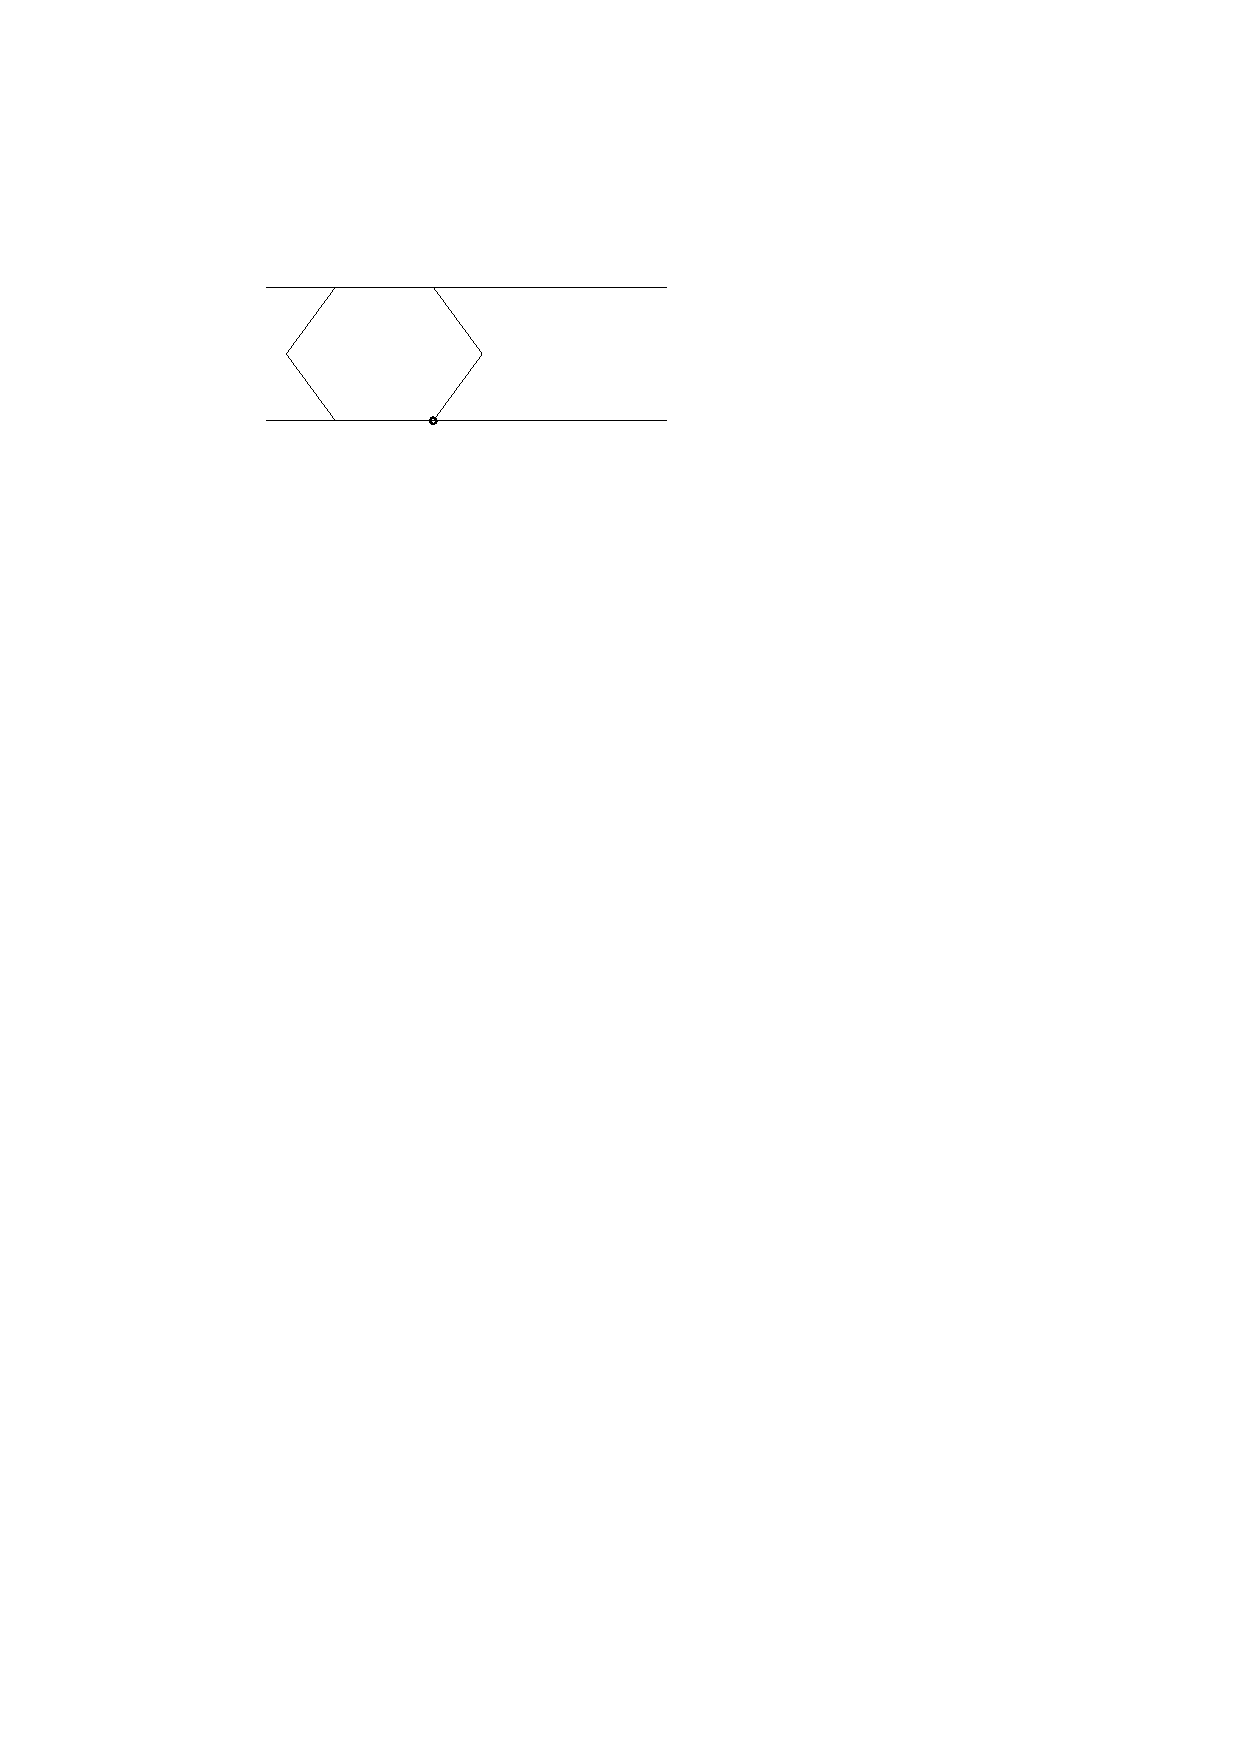
\includegraphics[width=\textwidth]{graphics/hexagonInChannelWithPinnedJointLeft.pdf}
	  \caption{The second realization of the hexagon residing in a channel with a pinned vertex.}
	  \label{fig:linkage-1-2}
  \end{subfigure}
\end{center} 
\caption{Due to the strip in the plane that the hexagon is bounded within the configuration space is limited to just two realizations.}\label{fig:linkage-1}
\end{figure}
So here we have a linkage whose conifguration space is limited to just two realizations.  With just two realizations, we can assign a binary value to them and have the linkage act as a boolean variable.  We will revisit this concept when we cover satisfiability problems later on in the paper.
\begin{figure}[h]
\begin{center}
  ~ %add desired spacing between images, e. g. ~, \quad, \qquad etc.
    %(or a blank line to force the subfigure onto a new line)
  \begin{subfigure}[b]{0.49\textwidth}
	  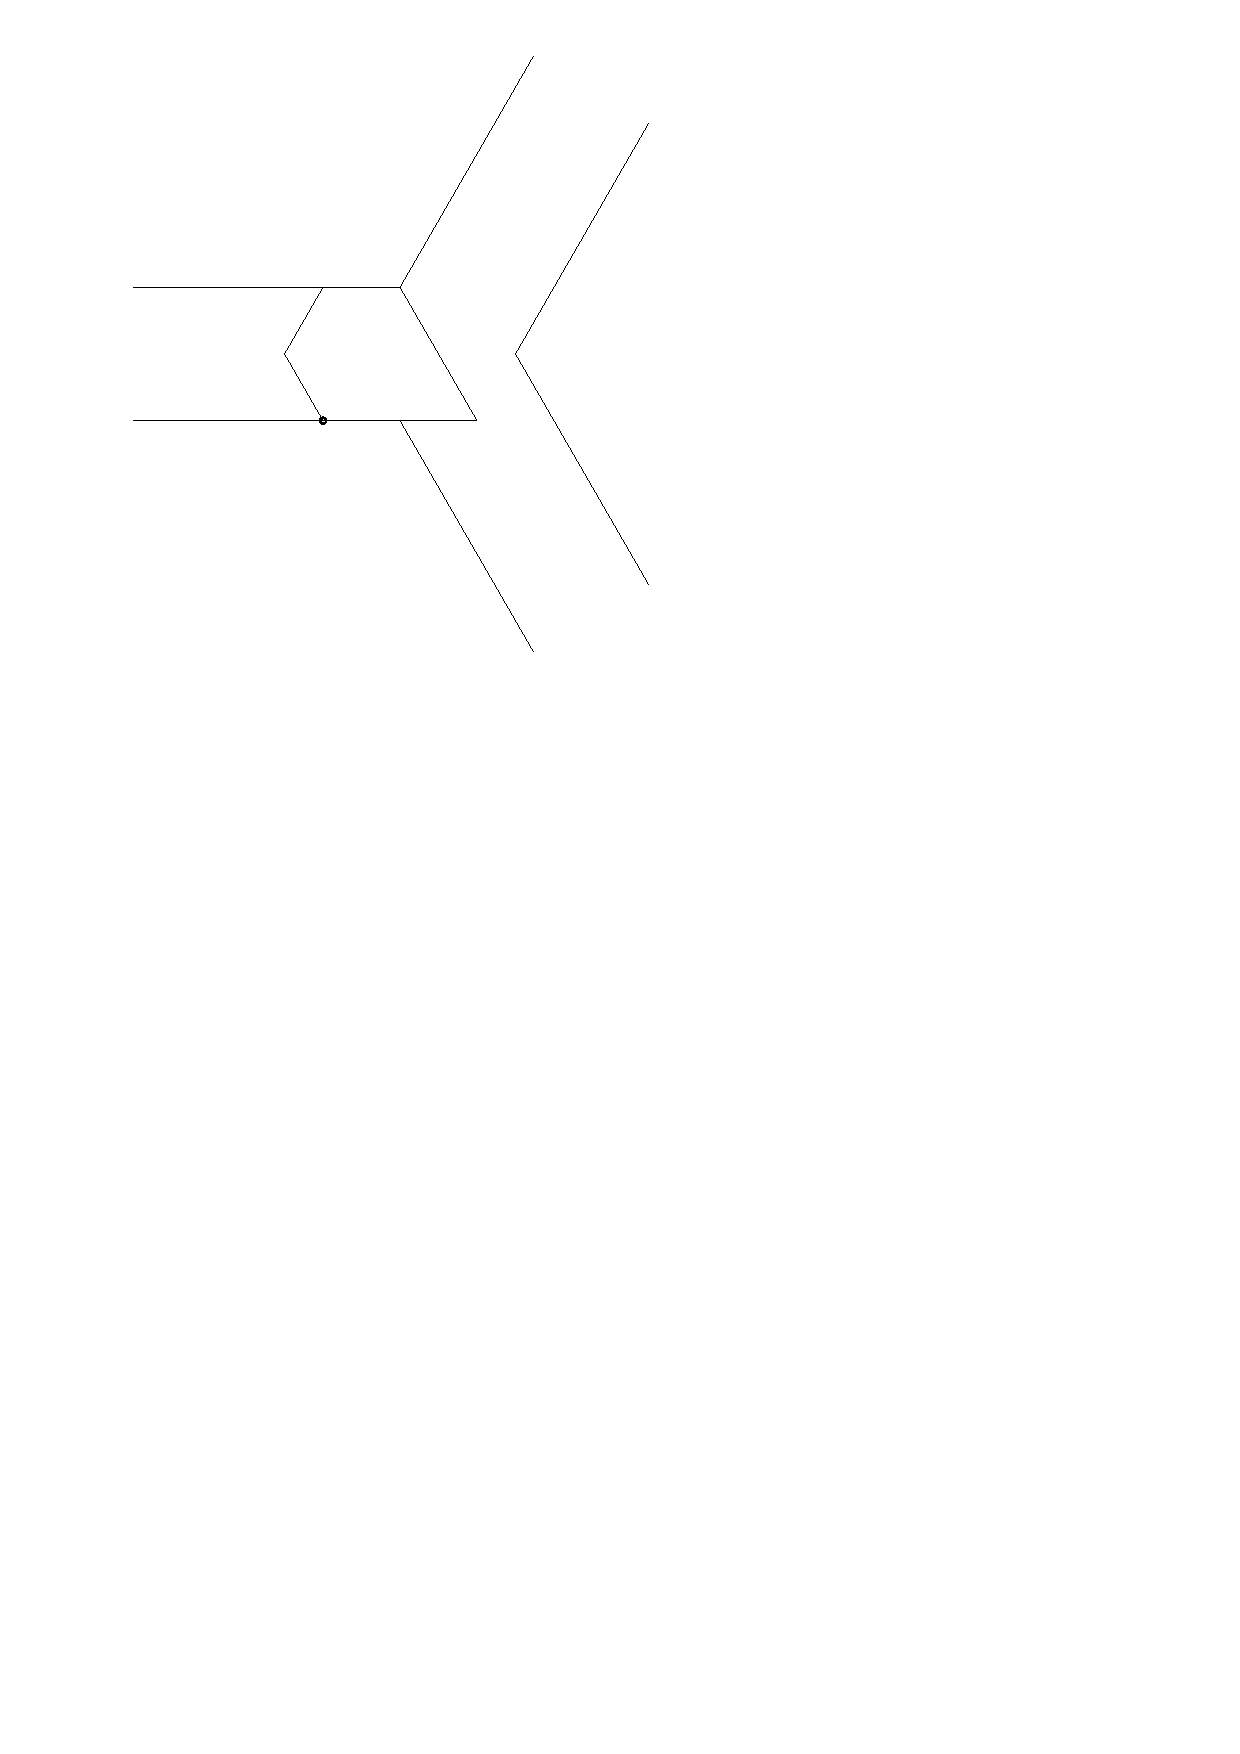
\includegraphics[width=\textwidth]{graphics/switchTerminalFinalized2.pdf}
	  \caption{A pentagon that is pinned in a channel junction that is formed by the sides of 3 large regular hexagons. It has two possible configurations, much like that of \ref{fig:linkage-1}}
	  \label{fig:linkage-2-1}
  \end{subfigure}
  \begin{subfigure}[b]{0.49\textwidth}
	  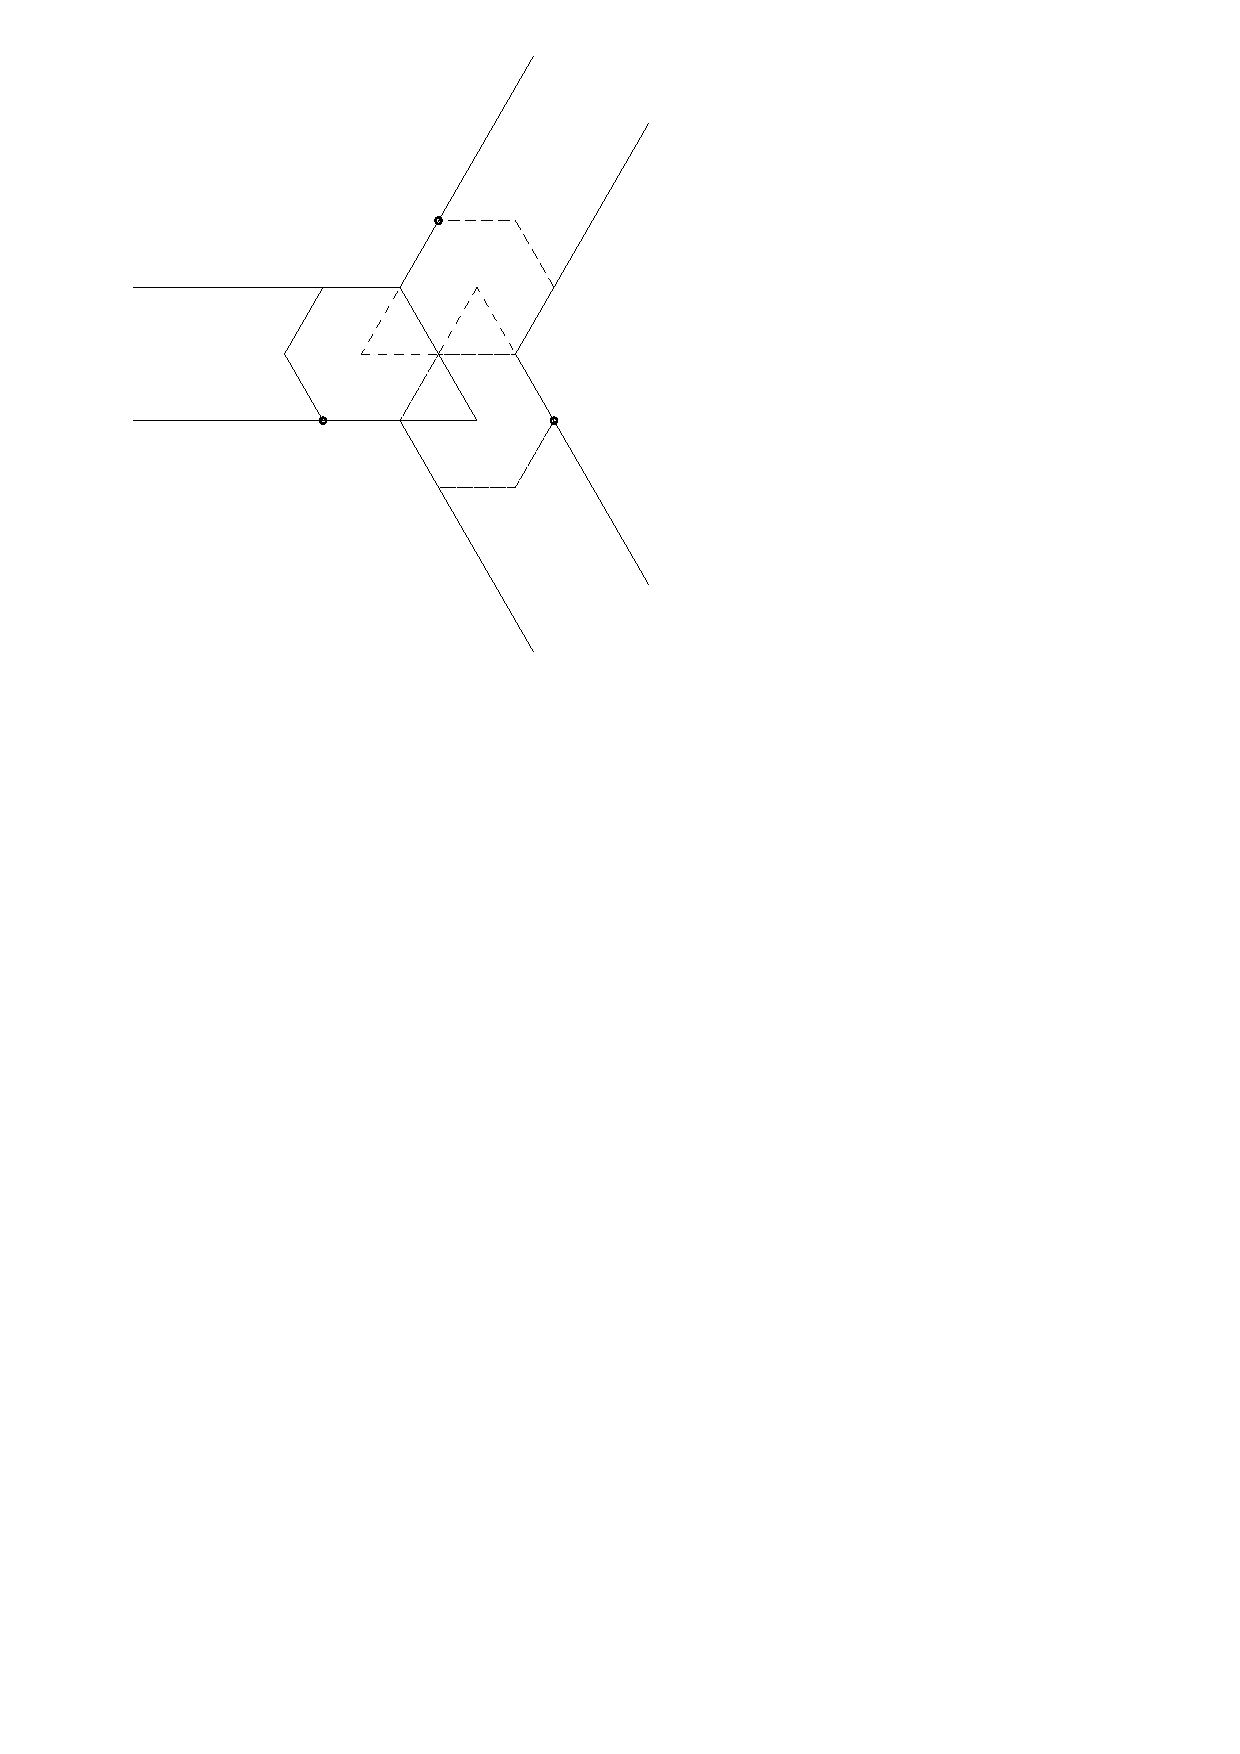
\includegraphics[width=\textwidth]{graphics/switchTerminalFinalized3.pdf}
	  \caption{A pinned pentagon residing in a channel junction that is formed by the sides of 3 large regular hexagons with 2 dashed pentagons intersecting it.}
	  \label{fig:linkage-2-2}
  \end{subfigure}
\caption{Suppose the channel formed is a junction of three regular hexagons.  The polygon partially residing in the junction is a regular hexagon with an equalateral triangle appended at an edge.  This polygon would prevent other polygons (i.e. the dashed polygons) of the same shape residing in the center of the channel without intersection. This demonstrates that a the configuration space within a multichannel environment can have concurrency issues, i.e. some configurations cannot be realizable.}
\end{center} \label{fig:linkage-2}
\end{figure}\newpage
Expanding upon the ideo of \ref{fig:linkage-1}, forming channels with junctions as shown in Figure \ref{fig:linkage-2} can be formed as such by evenly spacing the edges of a hexagonal lattice.  Visually, it is shown that only one of three possible pentagons can reside in the channel at one time.  By asserting certain conditions on the lattice, and extending the problem to a greater region of a hexagonal lattice, we will be able to pose a realizability problem of whether a configuration $\mathcal{A}$ can be reconfigured to $\mathcal{B}$ by switching pentagons without violating overlapped polygon conditions.
%Radius of regular polygons 
\newdimen\R
\R=3cm
\begin{figure}[h] 
\begin{center}
\begin{tikzpicture}
\begin{scope}
\filldraw[pattern=hexagons]  (0:\R) \foreach \x in {60,120,...,359} {
                -- (\x:\R)
            }-- cycle (90:\R);
\end{scope}
\end{tikzpicture}
\caption{A hexagonal lattice contained in a hexagon.}
\label{fig:lattice}
\end{center}
\end{figure}
\newpage
\subsubsection{Realizability of Linkages}
Suppose we had two configurations of a linkage, $\mathcal{A}$ and $\mathcal{B}$.  A question that can be posed is can we reconfigure $\mathcal{A}$ to $\mathcal{B}$ continuously while respecting simple planar graph conditions?  The answer to this question is a yes or no.  It has been shown that this problem can be posed as a planar satisfiability problem \cite{Breu19983,mulzer2008minimum} (Later on in this paper we'll cover satisfiability problems).  This is the type of problem that we face in this paper.  We will continue to explore this in a different manner, with circle packings.
% \begin{definition}[Graph]\label{def:linkages-2}
% An ordered pair $G = (V, E)$ comprising a set $V$ of vertices or nodes together with a set $E$ of edges or lines
% \end{definition} 
% \begin{definition}[Linkage]\label{def:linkages-1}
% A collection of fixed-length 1D segments joined at their endpoints to form a graph.
% \end{definition} 
% A linkage can be thought of as a type of path-connected graph, i.e. the segments of a linkage are the edges of a graph, and the endpoints of the segments are the vertices. For this paper, we restrict our self to linkages that are simple planar graphs, i.e. a linkage that:
% \begin{itemize}
% \item[\rn{1}] does not have multiple edges between any pair of vertices,
% \item[\rn{2}] does not have edges that cross, or
% \item[\rn{3}] have loops (i.e. $(v,v) \in E$).
% \end{itemize}  
% \begin{definition}[Cycle]\label{def:linkages-3}
%  A closed walk with no repetitions of vertices or edges allowed, other than the repetition of the starting and ending vertex
% \end{definition} 
% \begin{definition}[Configuration]\label{def:linkages-6}
% A specification of the location of all the link endpoints, link orientations and
% joint angles.\cite{demaine2008geometric}
% \end{definition}
% \begin{definition}[Configuration Space]\label{def:linkages-7}
% The space of all configurations of a linkage.
% \end{definition} 
% A configurations space is said to be continuous if for any two configurations, $\mathcal{A}$ and $\mathcal{B}$ of a linkage $L$, $\mathcal{A}$ can be continuously reconfigured to $\mathcal{B}$ such that, the reconfigurations reside in the configuration domain, $L$ remains rigid throughout reconfiguration (i.e. all links' lengths are preserved), and no violations of linkage intersection conditions. 
% \begin{definition}[Pinned Joint]\label{def:linkages-8}
% A vertex of a graph (or linkage) that is fixed to a position in a plane.
% \end{definition} 
% \begin{definition}[Free Joint]\label{def:linkages-8}
% A vertex of a graph (or linkage) that is not fixed to a position in a plane.
% \end{definition} 
% \begin{figure}[h]
% \begin{center}
% 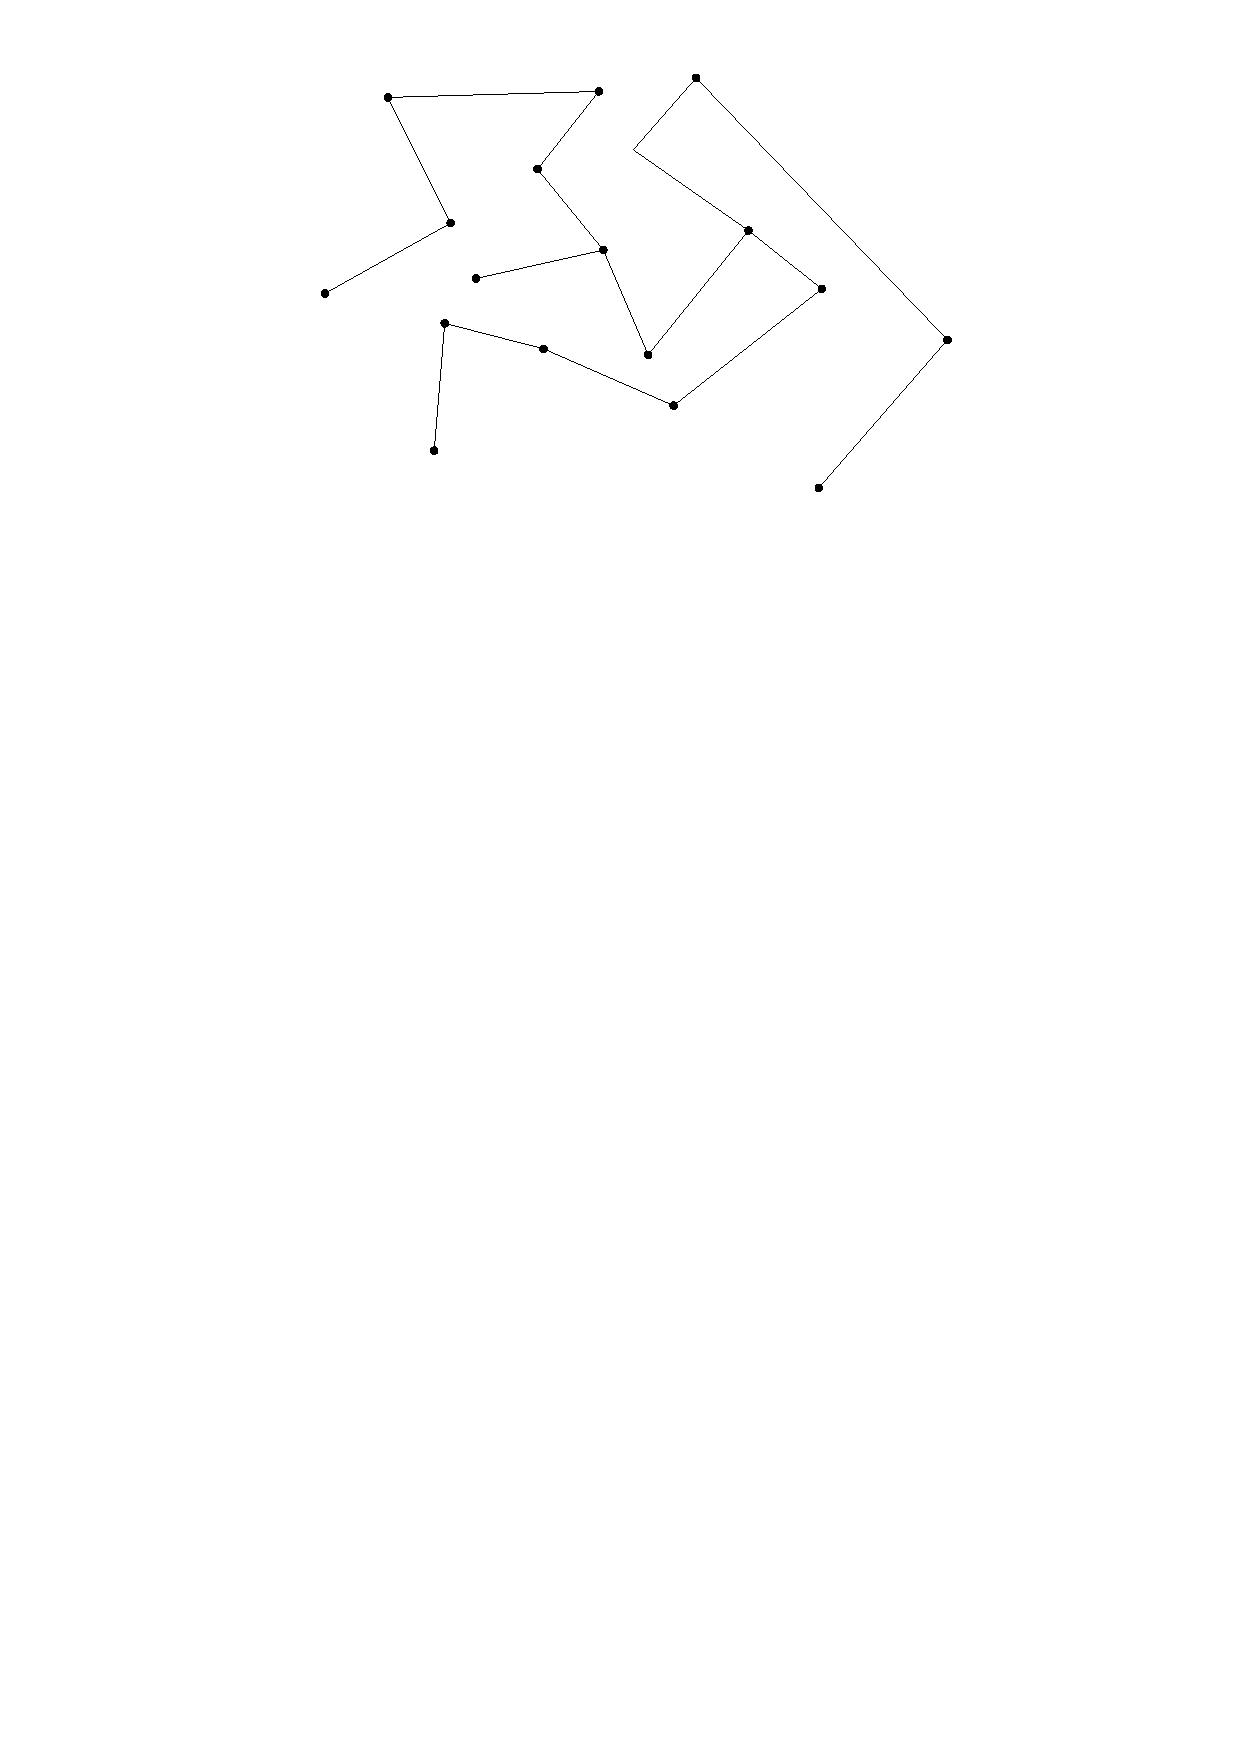
\includegraphics[scale=.5]{graphics/randomLinkage.pdf}
% \end{center} 
% \caption{A linkage with joints.}
% \end{figure} 
% \begin{figure}[h]
% \begin{center}
% 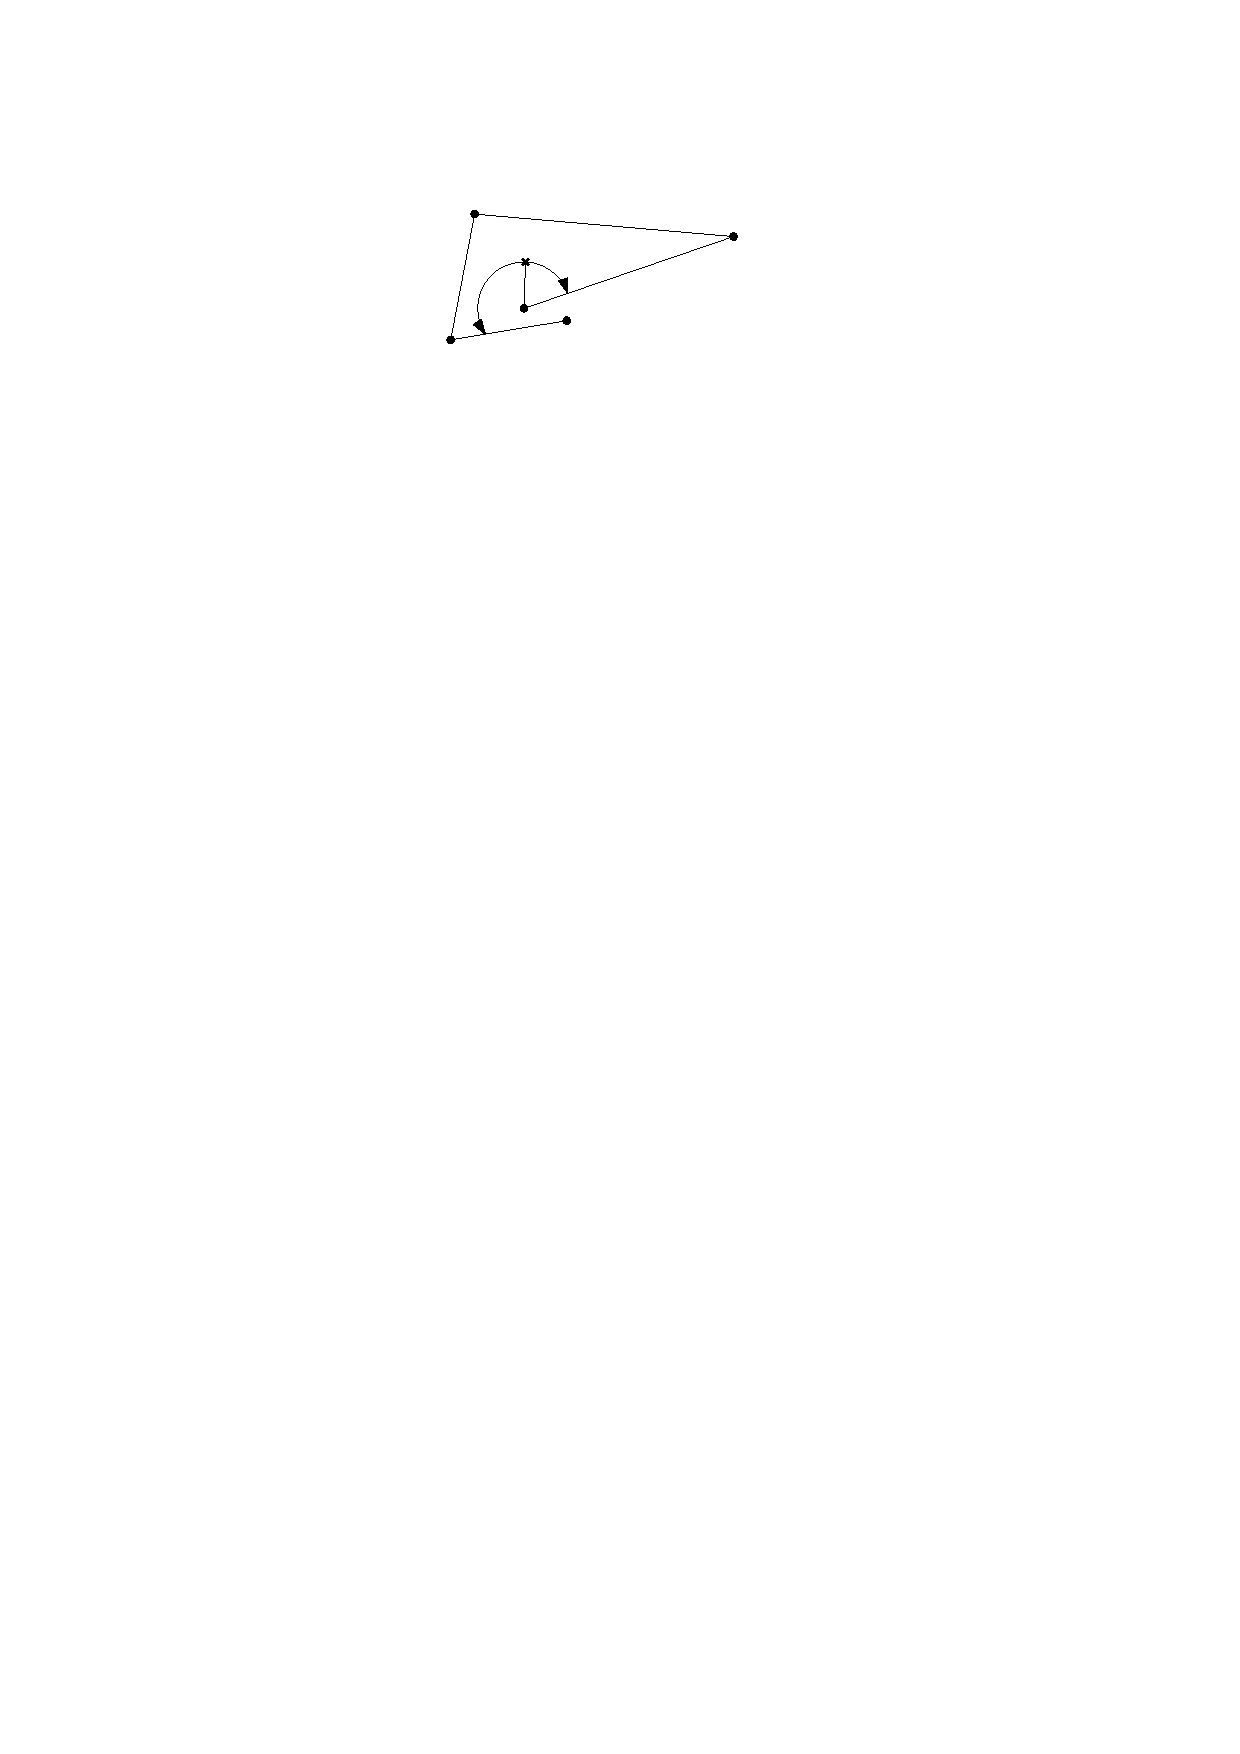
\includegraphics{graphics/freeJointPinnedJoint.pdf}
% \end{center} 
% \caption{The cross represents a free joint; the pinned joints are denoted as disks.  The range of motion shown by the arc describes the continous configuration space of the linkage.}
% \end{figure} 
% 
% For illustrations in the remainder of this paper, free joints will be represented as crosses and pinned joints will be represented as disks.

\section{Disk Arrangements}

\subsection{Oriented Realizations}
\subsection{Disk Packing Confinement Problem}
Consider the iterative problem:
\begin{enumerate}%1,2,3,4....
\item Start with a circle of diameter 1.
\item Add two kissing circles, each of diameter 1, that do not intersect with any other circle (they may kiss other
circles).
\item For each new kissing circle added, add two more non-intersecting kissing circles to it.
\end{enumerate} 
Figure (\ref{fig:circlePacking-1}) illustrates the iterative problem.  The problem with this is that the area in
which is necessary to contain this disk growing disk arrangement will exceed the area needed to contain it.
\begin{figure}[h]
\begin{center}
    %add desired spacing between images, e. g. ~, \quad, \qquad etc.
    %(or a blank line to force the subfigure onto a new line)
  \begin{subfigure}[b]{0.32\textwidth}
	  
\includegraphics[width=\textwidth]{graphics/degree2arrangement.pdf}
	  \caption{A disk arrangement with two layers of disks}
	  \label{fig:circlePacking1-1}
  \end{subfigure}
  \begin{subfigure}[b]{0.32\textwidth}
	  
\includegraphics[width=\textwidth]{graphics/degree3arrangement.pdf}
	  \caption{A disk arrangement with three layers of disks}
	  \label{fig:circlePacking1-2}
  \end{subfigure}
  \begin{subfigure}[b]{0.32\textwidth}
	  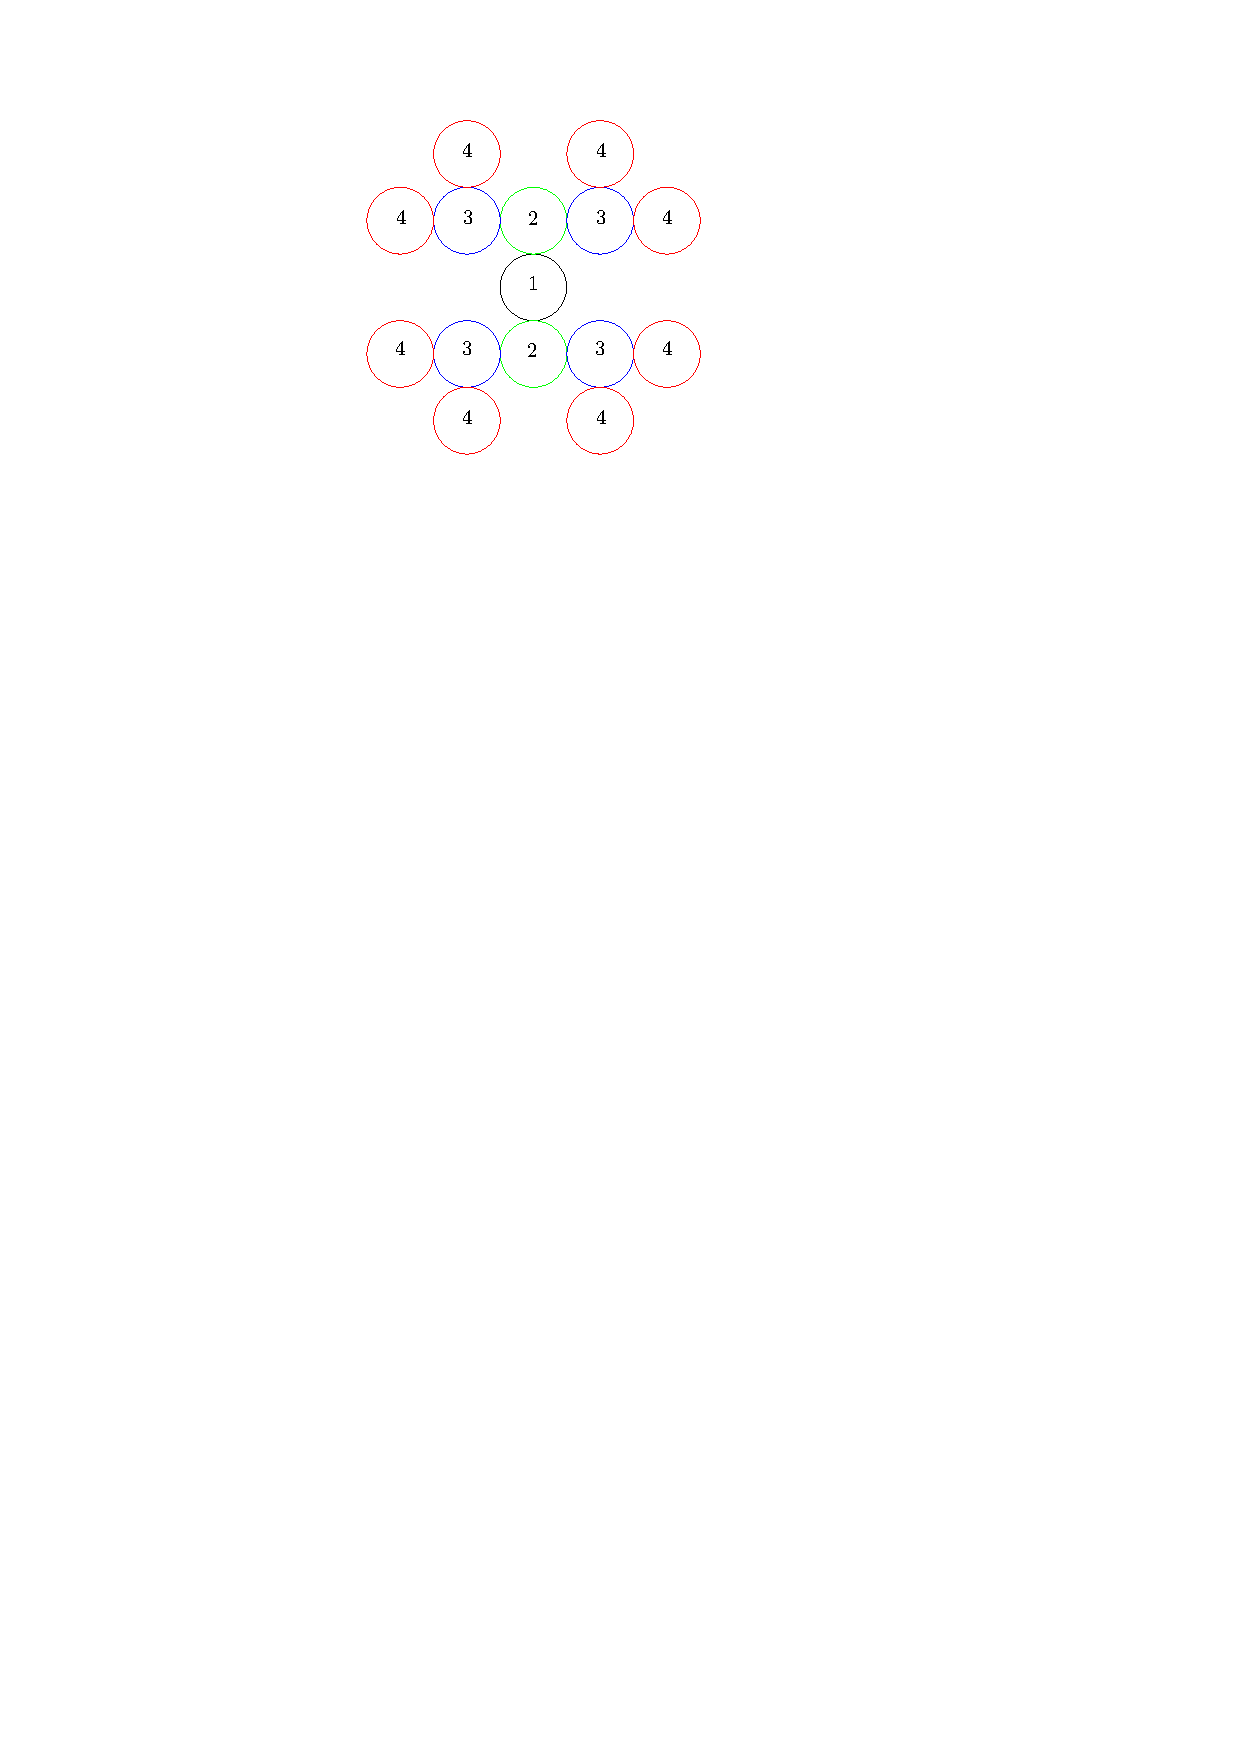
\includegraphics[width=\textwidth]{graphics/degree4arrangement.pdf}
	  \caption{A disk arrangement with four layers of disks}
	  \label{fig:circlePacking1-3}
  \end{subfigure}
\end{center} 
\caption{The gradual growth of disk arrangements by adding two kissing disks to each of the previously generated disks.  By continuing this arrangement growth, the space needed to contain the kissing disks will exceed the area containing the disk arrangements.}\label{fig:circlePacking-1}
\end{figure}
\begin{tabular}{}
n&
\end{tabular} 
\section{Satisfiability}
\begin{prob}[Satisfiability Problem]\label{prob:Satisfiability-1}%Problem/Question
Let $\left\lbrace x_i \right\rbrace_{i=1}^{n} $ be boolean variables, and $t_i \in \left\lbrace 
x_i\right\rbrace_{i=1}^{n}  \cup \left\lbrace \bar{x}_i\right\rbrace_{i=1}^{n}   $.  A 
\textit{clause} is is said to be a disjuction of distinct terms:
$$
t_1 \vee \cdots \vee t_{j_k} = C_k
$$
Then the \textit{satisfiability problem} is the decidability of a conjuction of a set of clauses, 
i.e.:
$$ \wedge_{i=1}^m C_i$$
\end{prob} \cite{skiena2009algorithm}
A \textit{3-SAT problem} is a SAT problem with all clauses having only three boolean variables. 
\begin{definition}[Planar 3-SAT Problem]\label{def:Satisfiability-2}
Given a boolean 3-SAT formula $B$, define the associated graph of $B$ as follows:  
\begin{equation}\label{eqn:sat-1}
G(B) = \left(\set{v_x}{v_x\text{ represents a variable in }B} \cup \set{v_C}{v_C\text{ represent a 
clause in }B}  , \set{\left( v_x, v_C\right) }{x \in C \text{ or } \bar{x} \in C}  \right) 
\end{equation} 
If $G(B)$ in equation (\ref{eqn:sat-1}) is planar, then $B$ is said to be a \textit{Planar 3-SAT 
Problem} \cite{mulzer2008minimum}.
\end{definition}
\subsection{Logic Engine}
The logic engine simulates the well known Not All Equal 3 SAT Problem (NAE3SAT).  
\subsection{Not All Equal 3 SAT Problem}
\begin{prob}[Satisfiability Problem]\label{prob:Satisfiability-2}%Problem/Question
Give a set of clauses $C$, each containing three boolean variables, can each clause contain at 
least one true variable and one false variable?
\end{prob}
%Universality component
%encoding the engine
\subsubsection{Construction of the Logic Engine}
The components of the logic engine are as follows: the rigid frame, the shaft, the armatures, 
the chains, and the flags.  The \textit{rigid frame} is a rectangular enclosure with a horizontal 
shaft place at mid-height.  The \textit{armatures} are concentric rectangular frames contained 
within the rigid frame.  Each armature can rotate about the shaft; other motions on the armature 
are disallowed.  Given an NAE3SAT, for each variable there is a corresponding armature. On each 
armature, there are chains.  A pair of \textit{chains}, $a_j$ and $\bar{a}_j$ correspond to the 
variable $x_j$ and $\bar{x}_j$ respectively.  The pair is placed on each armature, reflected at a 
height of $h$ above and below the shaft, i.e. one place above the shave at a height of $h$, the 
other placed below the shaft at a height of $-h$.
%insert an armature graphic

\subsection{Encoding the Logic Engine}
For each clause of an NAE3SAT, there exists a set of corresponding chains, namely the $h^\text{th}$ 
clause is the set of chains on the armatures at the $h^\text{th}$ row above and below the shaft. A 
chain is \textit{flagged} if the corresponding variable resides within the clause.  The flag can 
point in either the left or right directions indicating a truth assignment for that variable within 
the clause.  A flag is attached to the $i^\text{th}$ chain of every $a_j^\text{th}$ and 
$\bar{a}_j^\text{th}$ chain with the following exceptions:
\begin{enumerate}
 \item if the variable $x_j$  is in clause $C_i$, then link $i$ of $a_j$ is unflagged,
 \item if the variable $\bar{x}_j$ is in clause $C_i$, then link $i$ of $a_j$ is unflagged.
\end{enumerate}
\begin{thm}\label{thm:Satisfiability-1}
 An instance of $NAE3SAT$ is a ``yes'' instance if and only if the corresponding logic engine has a 
flat, collision-free configuration.
\end{thm}
\begin{pf}
 If an instance of $NAE3SAT$ is a ``yes'', then every clause in $C$ contains at least one true 
variable and one false variable.  Now suppose the following truth assignment:
\begin{equation}\label{eqn:Satisfiability-1}
 t\left( x_j \right) = \left\lbrace\begin{array}{cr}
  1 & x_j\text{ and }\bar{x}_j \text{are placed at the top and bottom respectively}\\
  0 & x_j\text{ and }\bar{x}_j \text{are placed at the bottom and top respectively}\\
 \end{array}\right.
\end{equation}
For each clause $c_i \in C$, there exists a variables in $c_i$ such that $t\left( y_i \right) = 1$ 
and $t\left( z_i \right) = 0$.  This implies that there exists an unflagged chain in the 
$i^\text{th}$ and $-i^\text{th}$ row of the frame.  To avoid a collision in each row, trigger the 
flags to point towards the unflagged link. Thus, the corresponding logic engine has a 
flat, collision-free configuration.

If the corresponding logic engine has a flat, collision-free configuration, then there must exist 
an unflagged link in each row.  Without loss of generality, we have that the variables $y_j$ and 
$z_i$ is in clause $C_i$ such that $t\left( y_i \right) = 1$ and $t\left( z_i \right) = 0$ for each 
$i$.  Thus, we have an instance of $NAE3SAT$ is a ``yes'' instance. \cite{BET+99}
\end{pf}


%\subsection{Disk Arrangements}

% Here goes something
% % \begin{figure}[htbp]
% % \begin{center}
% % 
\includegraphics{graphics/RightSwitchBetweenTwoPolygons.pdf}
% % \caption{blah blah blah}
% % \end{center} 
% % \end{figure} 
% % \begin{figure}[htbp]
% % \begin{center}
% % 
\includegraphics{graphics/LeftSwitchBetweenTwoPolygons.pdf}
% % \caption{blah blah blah}
% % \end{center} 
% % \end{figure} 
% \begin{figure}[h]
% \begin{center}
%   ~ %add desired spacing between images, e. g. ~, \quad, \qquad etc.
%     %(or a blank line to force the subfigure onto a new line)
%   \begin{subfigure}[b]{0.45\textwidth}
% 	  
\includegraphics[width=\textwidth]{graphics/RightSwitchBetweenTwoPolygons.pdf}
% 	  \caption{blah blah blah}
% 	  \label{fig:linkage-1-1}
%   \end{subfigure}
%   \begin{subfigure}[b]{0.45\textwidth}
% 	  
\includegraphics[width=\textwidth]{graphics/LeftSwitchBetweenTwoPolygons.pdf}
% 	  \caption{blah blah blah}
% 	  \label{fig:circlePacking1-2}
%   \end{subfigure}
% \end{center} 
% \caption{Due to the strip in the plane that the hexagon is bounded within the configuration space is limited to just two realizations.}\label{fig:circlePacking-1}
% \end{figure}
% \subsection{Circle Packing}
% 
% 
% Any circle embedded in a plane has a given center point and radius.  This information of planar embedded circle packings allows us to establish the relationship to linkages with the following construction:
% \begin{itemize}
% \item[\rn{1}] let the centerpoints of the circle packing be a set of vertices $V$;
% \item[\rn{2}] if two circles in a circle packing are tangent, we define an edge between their centerpoints.  The distance of this edge is the sum the radii of the two tangent circles.
% \end{itemize}  
% This construction establishes a relationship between linkages and circle packings.  It begs questioning as to whether every connected simple planar graph has a circle packing.  The question is answered in the following theorem.
% 
% 
% 
% 
% A proof of Theorem \ref{thm2-1} is found in chapter 7 of \cite{stephenson2005introduction}.  Theorem \ref{thm2-1} also gives us the ability to establish an equivalent definition of configuration spaces on circle packings and allows us to pose the same realizability problems found with simple planar graphs.  To narrow the focus of the types of circle packing realizabilty problems that we are interested in, we add the following restriction: all circles in a circle packing have unit diameter. 
% \subsubsection{Realizability Problems in Unit Disk Packings}
% In \cite{Breu19983}, it was shown that unit disk graph recognition is NP-Hard. 
% \subsection{Area Packing Problem}
% 
% 
% % \begin{definition}[Circle Packing]\label{def:circlePacking}
% % $P$ of a planar graph $G$ is a set of of circles with disjoint
% % interiors $\left\lbrace C_v \right\rbrace_{v \in G} $ such that two
% % circles are tangent if and only if the corresponding vertices form an edge.
% % \cite{arXiv13113363v1}
% % \end{definition} 
% % \begin{thm}[Circle Packing Theorem]\label{thm2-1}
% % For every connected simple planar graph $G$ there is a circle packing in the
% % plane whose intersection graph is (isomorphic to) $G$.
% % \end{thm}
% % \begin{figure}[!ht]
% % \begin{center}
% % 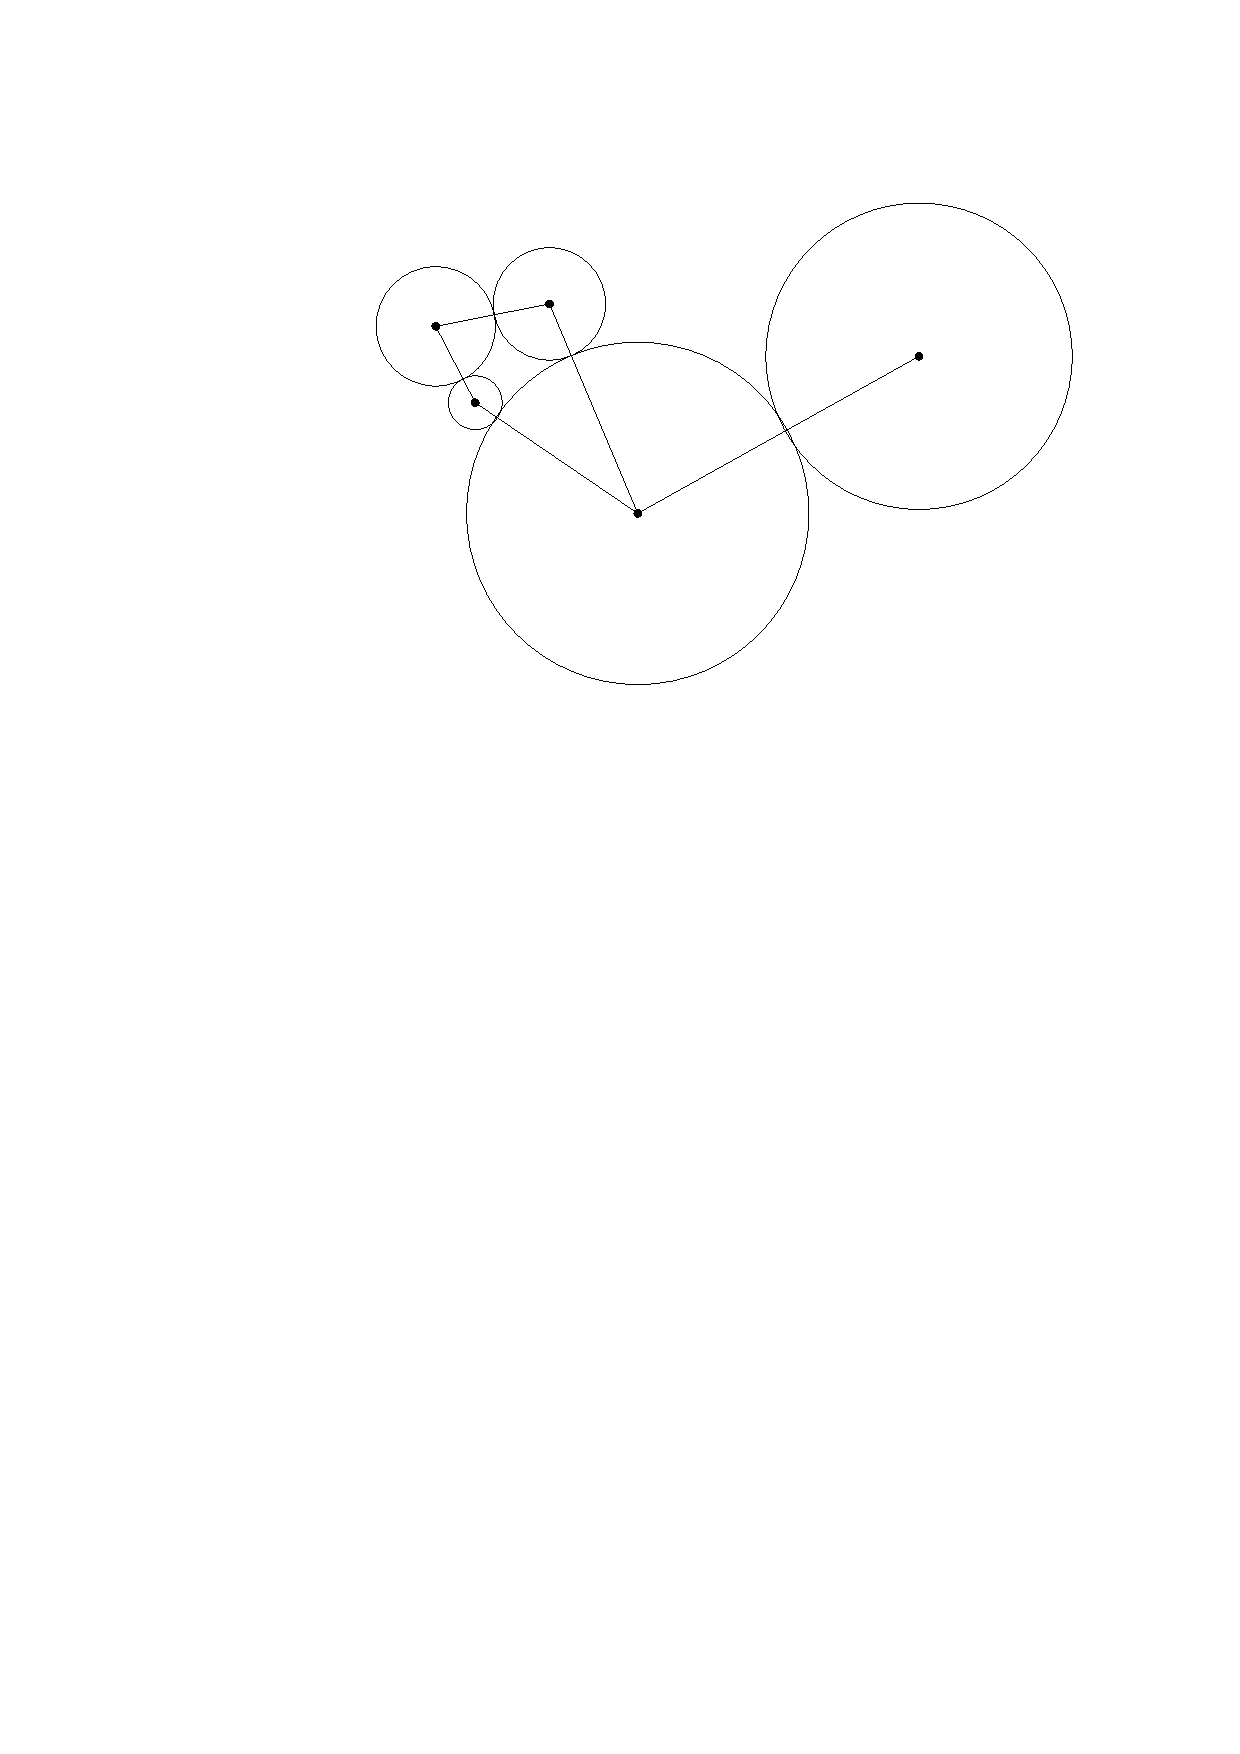
\includegraphics[scale=.5]{graphics/circlePackingTheoremExample.pdf}
% % \end{center} 
% % \caption{This figure is an example of a circle packing for the given simple planar graph.}
% % \end{figure} 
% % A proof of Theorem \ref{thm2-1} is found in \cite{stephenson2005introduction}.
% % 
% % \subsubsection{Circle Packings and Polygonal Linkages}
% % Given a circle of radius $r$ and its center point, $(x,y)$, we establish the isomorphism  to a hexagon by
% % circumscribing the vertices of the regular hexagon.
% % \begin{figure}[h]
% % \begin{center}
% % 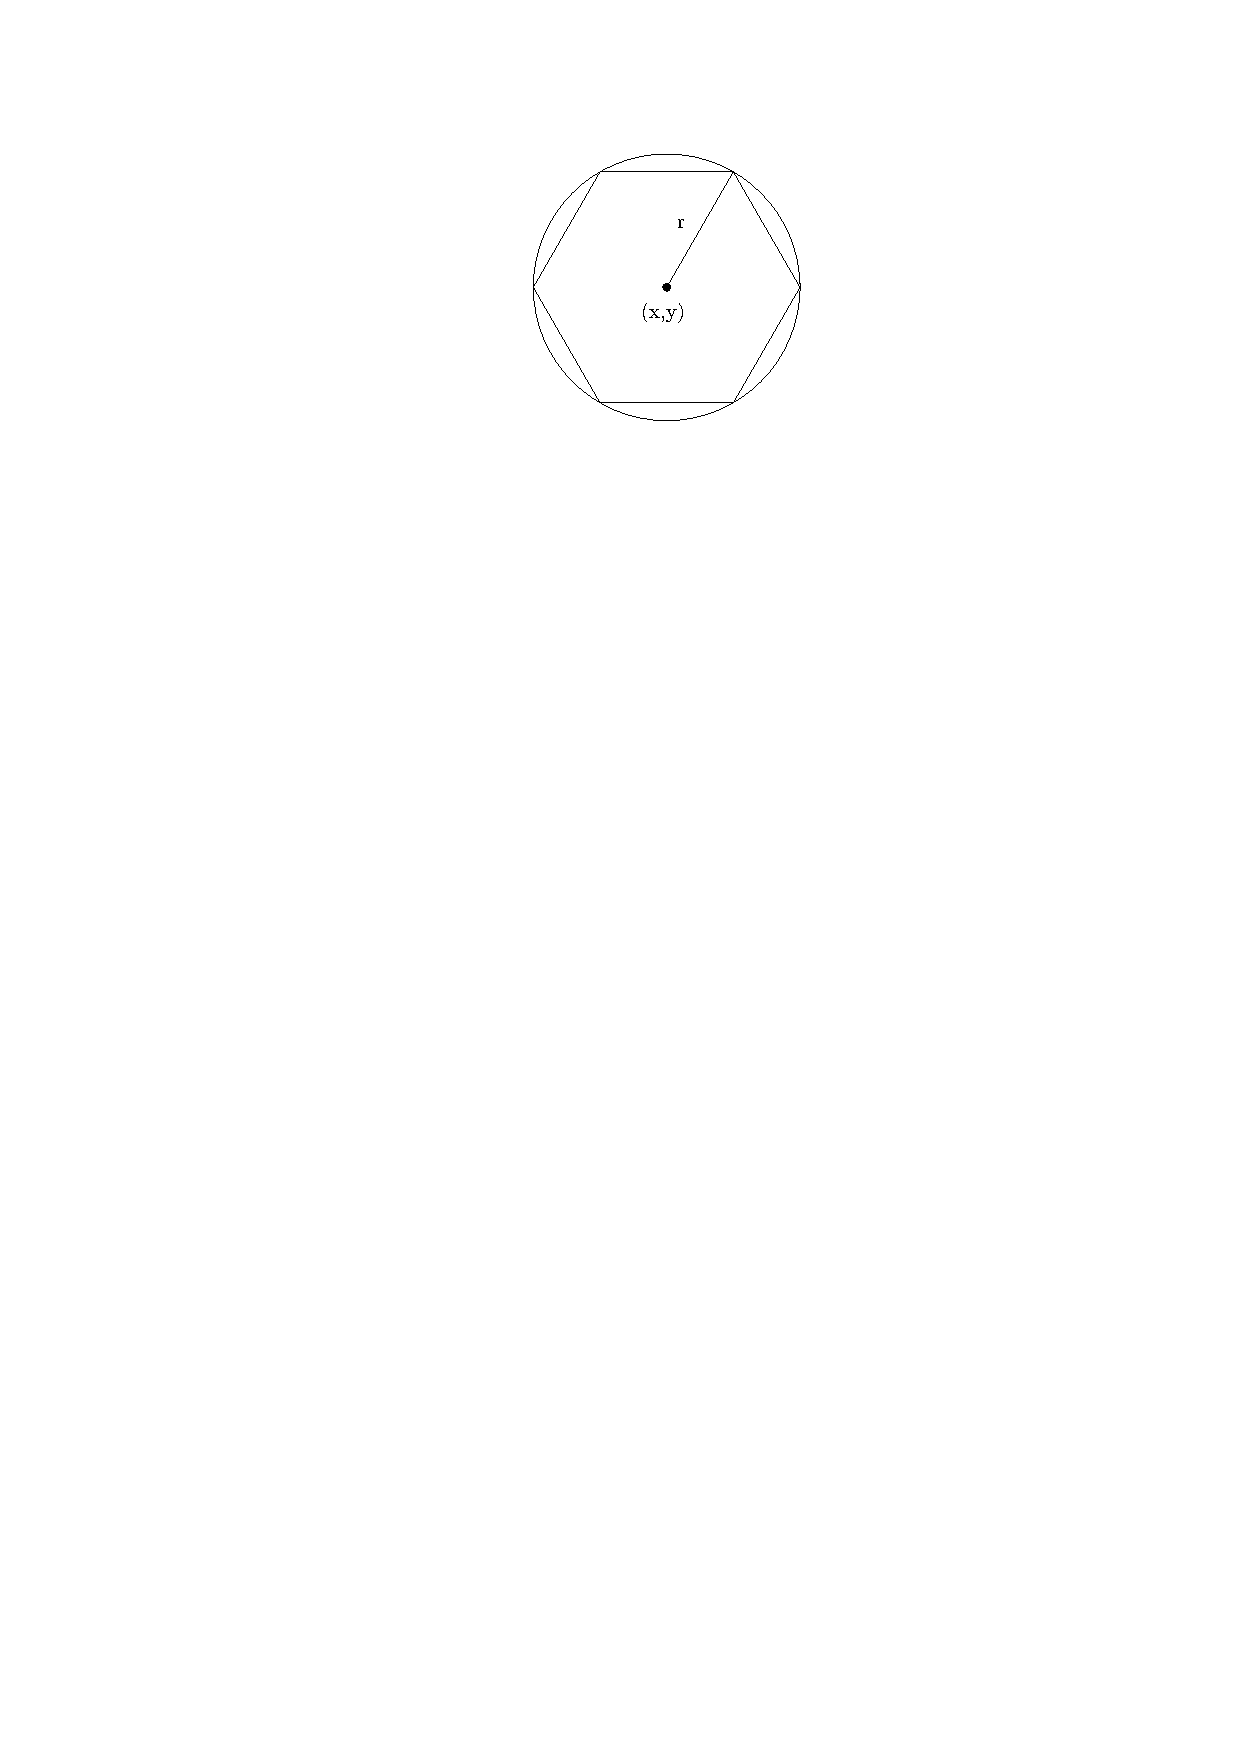
\includegraphics{graphics/circumscribedHexagon.pdf}
% % \caption{A circumbscribed hexagon}
% % \end{center}
% % \end{figure}
% \subsubsection{Hinged Polygons}
% \begin{definition}[Polygonal Chain]\label{def}
% A polygonal chain $P = \left( v_0, v_1, \dots, v_{n-1}\right) $ is a sequence of
% consecutively joined segments (or edges) $e_i = v_i v_{i+1}$ of fixed lengths
% $l_i = \left\vert e_i\right\vert $, in a plane. \cite{Biedl99lockedand}
% \end{definition}
% A chain is said to be closed if $v_{n-1} = v_1$, otherwise it is said to be
% open. Hinged polygons have been researched for decades and related to linkage problems
% \cite{Biedl99lockedand,canny1988complexity}.
% 
% Consider the locked configuration of figure \ref{figure:7hexLocked}.  We can
%  configure the hexagons to be locked by placing hinged points as follows:
% \begin{figure}[!ht]
% \begin{center}
% 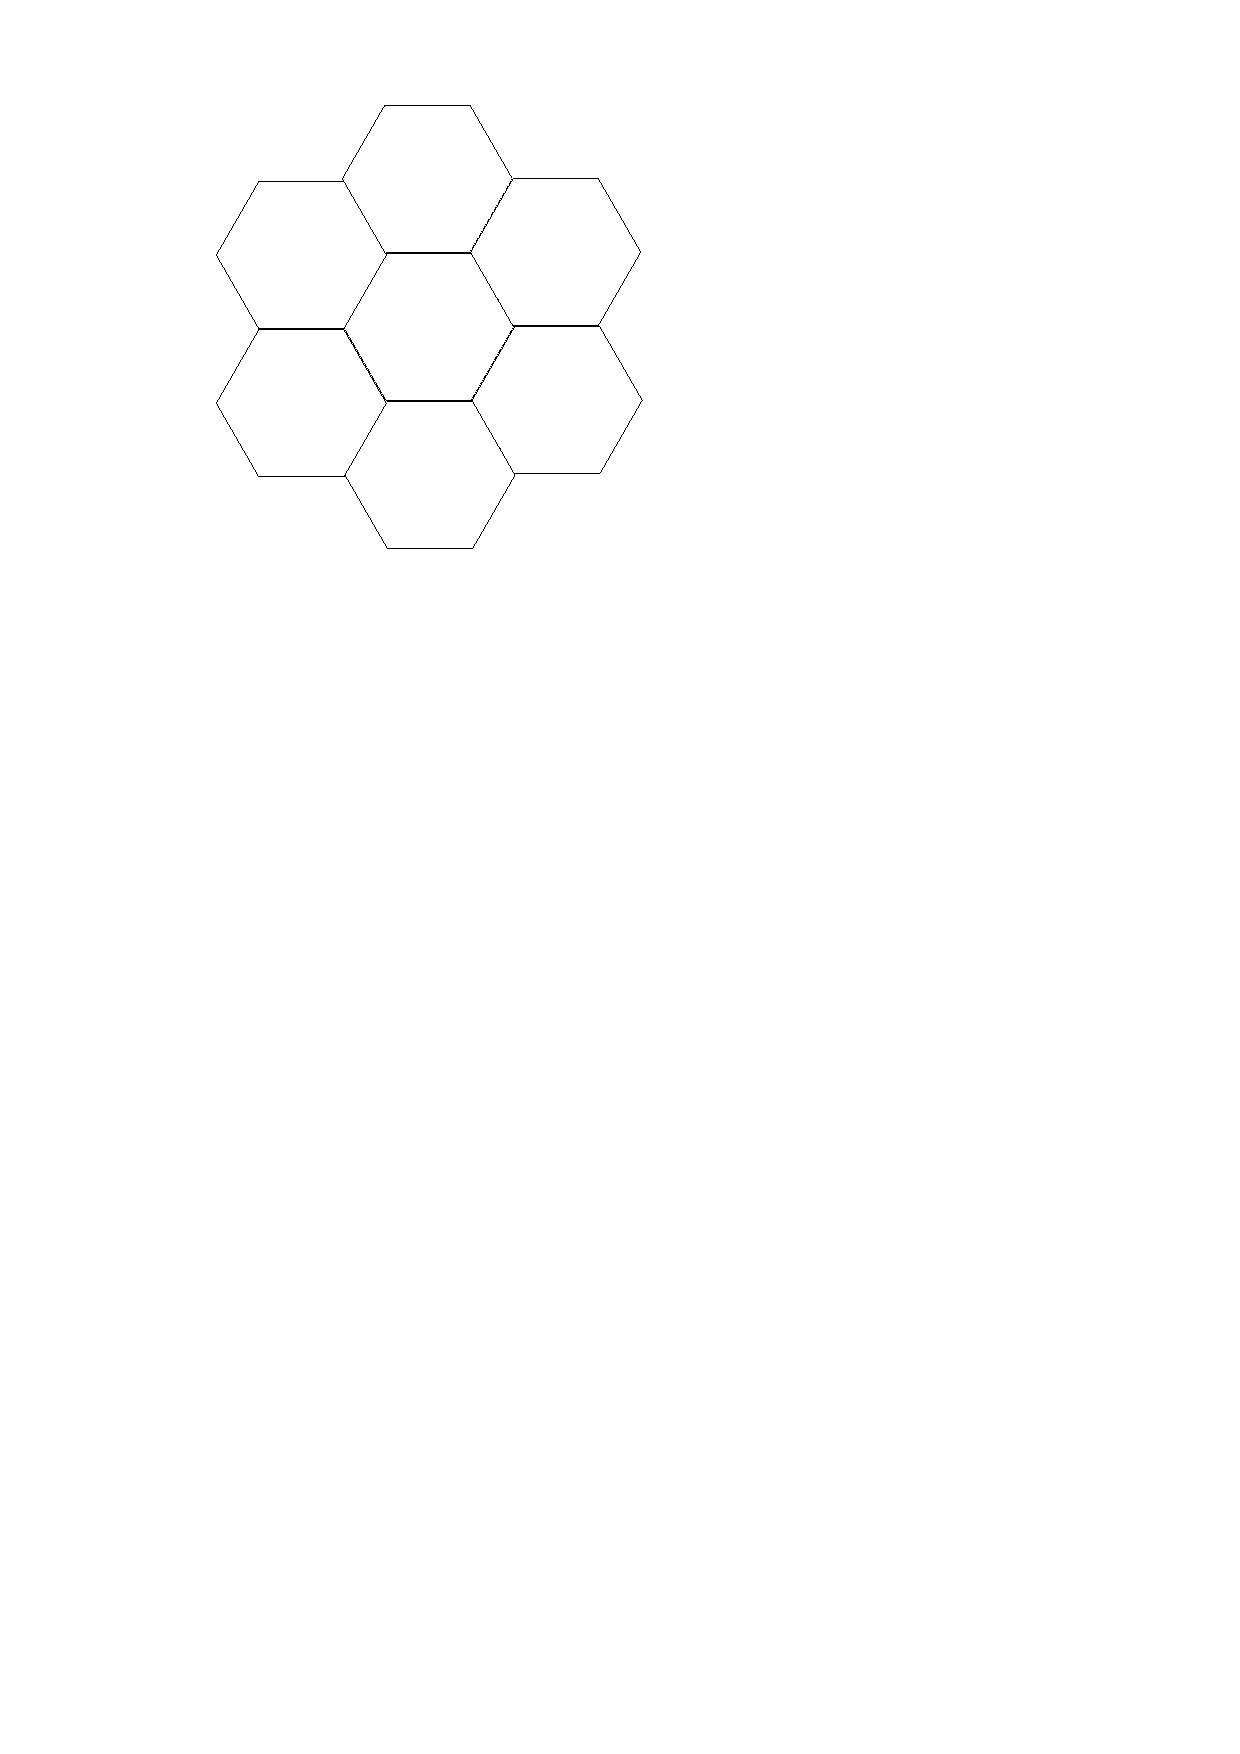
\includegraphics[scale=.33]{graphics/7hexLocked.pdf}
% \caption{A locked 7 hexagonal configuration.  (needs to modify picture by
% placing red points for hing points.)}
% \label{figure:7hexLocked}
% \end{center} 
% \end{figure}
% 
% \subsubsection{Hinged Hexagons of Fixed Size}
% 
% \paragraph{The Shapes}
% Figure \ref{fig:lockingShape} is a locking shape:
% % \begin{figure}[h]
% % \begin{center}
% % 
\includegraphics{graphics/lockingShape.pdf}
% % \caption{This is the shape that resides in boundary of the lattice.}
% % \label{fig:lockingShape}
% % \end{center}
% % \end{figure}
% \begin{figure}[h]
% \begin{center}
% 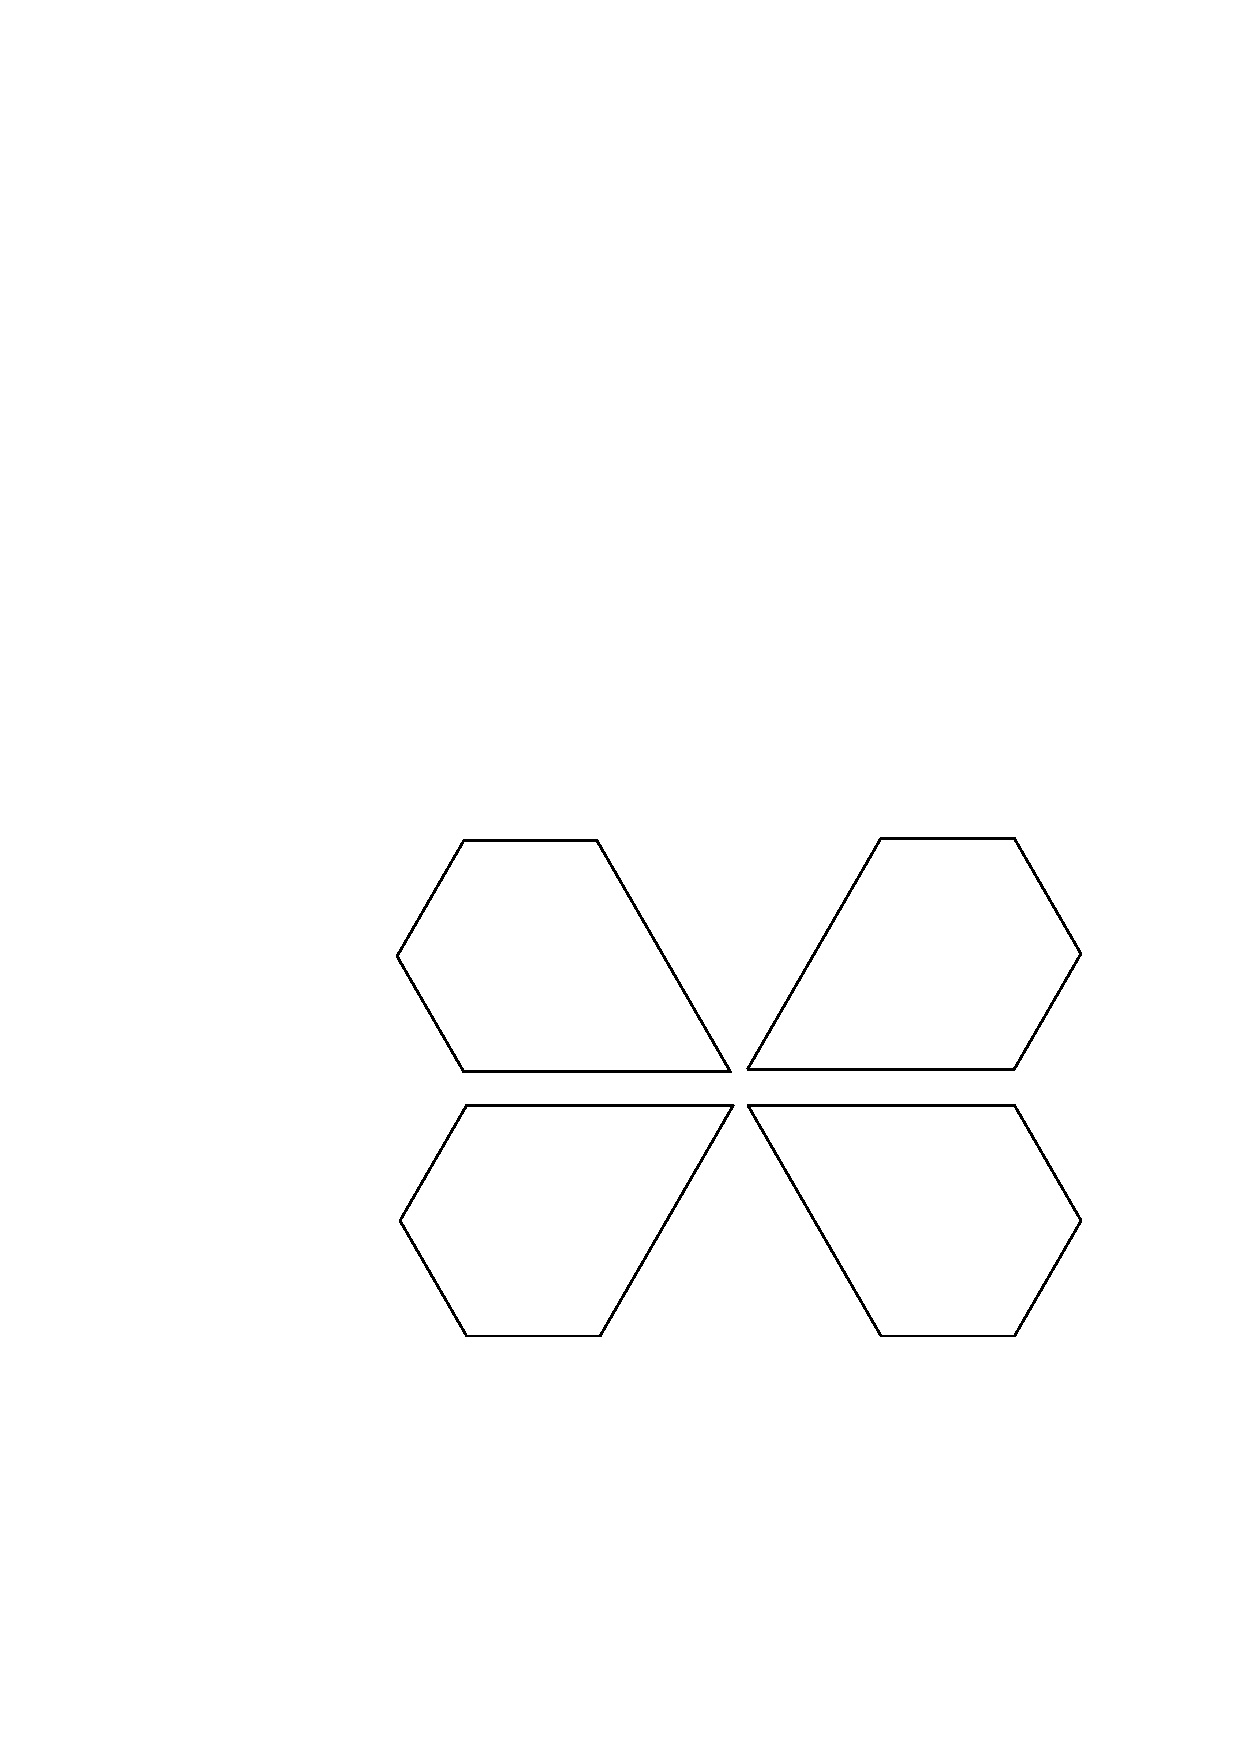
\includegraphics[scale=.33]{graphics/shapeInChannel.pdf}
% \end{center} 
% \caption{A locking shape in the lattice boundary's channel.}
% \label{fig:lockingShape}
% \end{figure}
% Figure \ref{fig:lockingShape} shall reside in the boundary of a lattice and have
% a hinge point at one vertex where the locking shape and boundary meet.
% 
% \paragraph{Junctions}
% We define junctions to be the point three hexagons meet in a hexagonal lattice,
% e.g. Figure \ref{fig:lattice}.
% %Radius of regular polygons 
% \newdimen\R
% \R=4.5cm
% \begin{figure}[h] 
% \begin{center}
% \begin{tikzpicture}
% \begin{scope}
% \filldraw[pattern=hexagons]  (0:\R) \foreach \x in {60,120,...,359} {
%                 -- (\x:\R)
%             }-- cycle (90:\R);
% \end{scope}
% \end{tikzpicture}
% \caption{A portion of a hexagonal lattice.}
% \label{fig:lattice}
% \end{center}
% \end{figure}
% \newpage
% \paragraph{Central Scaling}
% \paragraph{Junctions in Conjunctive Normal Form}
% Explain the configurations we're interested in.

\nocite{demaine2008geometric,frederickson1997dissections,stephenson2005introduction}
\bibliographystyle{plain}
\bibliography{bibliography}
\end{document}